% !TEX program = pdflatex
% !TEX enableSynctex = true
% !BIB program = bibtex

\documentclass[12pt]{article}

\usepackage{setspace}
\usepackage{amsmath}
\usepackage{amsfonts}
\usepackage{graphicx}
\usepackage{float}
\usepackage{dsfont}
\usepackage{natbib}
\addtolength{\oddsidemargin}{-.7in}
\addtolength{\evensidemargin}{-.7in}
\addtolength{\textwidth}{1.4in}
\usepackage{enumerate}
\onehalfspacing
\usepackage{geometry} % Required for customizing page layout
\usepackage{ragged2e}

\usepackage{caption}
\usepackage{booktabs}

\usepackage{hyperref}
\hypersetup{
	pdfstartview = FitH,
	pdfauthor = {...},
	pdftitle = {...},
	pdfkeywords = {...; ...; ...; ...},
	colorlinks = true,
	linkcolor = blue,
	urlcolor = blue,
	citecolor = blue,
	linktocpage=true
}

\DeclareMathOperator{\E}{\mathbb{E}}
\DeclareMathOperator*{\argmax}{arg\,max}
\DeclareMathOperator*{\argmin}{arg\,min}
\hbadness=10000

\title{Reorganizing Debt Finance: How Bankruptcy Regimes Shape Access to Cash Flow-Based Debt}
\date{}

\begin{document}

\author{Barnabás Székely}
\date{\today}
\vspace{-1in}

\maketitle

\begin{abstract}
\noindent

This paper argues that reorganization costs raise liquidation risks and limit access to cash flow-based debt for small but productive firms, which has significant consequences for broader macroeconomic outcomes. Creditors restrict lending against future cash flows if they expect the borrower to be liquidated under financial distress. This puts moderately-sized firms at a disadvantage, as the administrative and time costs of reorganization often force the liquidation of these businesses. Small but productive firms have inadequate access to cash flow-based debt finance, which suppresses entry rates and yields aggregate productivity losses. However, streamlining the reorganization process can mitigate this source of misallocation. I find that reducing reorganization costs can considerably improve aggregate productivity through limiting liquidation risk and improving access to cash flow-based debt. 

\bigskip{}
\bigskip{}
%\bigskip{}
%\bigskip{}
%\vspace{-0.5cm}

Keywords: Heterogeneous firms, Credit market frictions, Cash flow-based lending, SME financing
\medskip{}
% JEL Classification Code: E32, C22, E27.
\end{abstract}
\thispagestyle{empty}

\pagebreak{}


\section{Introduction \label{sec:introduction}} 

Collateral constraints represent major barriers to firm growth (Beck et al., 2006; Schmalz et al., 2017, Catherine et al., 2021). Borrowing limits defined by the value of collateralizable assets can be particularly restrictive, since these create self-perpetuating cycle: limited collateral restricts access to external finance, which in turn limits firm growth and delays the accumulation of collateral.\footnote{This notion traces back to Bernanke et al. (1999), originally applied to credit cycles, but it extends across the life cycles of firms as well.} Cash flow-based debt contracts allow firms to borrow against future cash flows rather than specific physical assets (Lian and Ma, 2021). This form of lending could, in principle, alleviate collateral constraints for small, but productive firms as it evaluates future earning potential rather than the accumulated collateral. However, for moderately-sized firms, borrowing against future cash flows (CF-based debt) remains significantly more expensive than borrowing against physical assets (asset-based debt).\footnote{US non-financial corporations under $100$M USD of assets pay an average credit spread of $7.19\%$ on CF debt and only $5.25\%$ on AB-debt. This result is robust to multivariate analysis. For the same set of firms, CF-based debt is associated with a 0.8pp higher spread (S\$P Capital IQ).}  \vspace{3mm}  \\
In this paper, I argue that a key factor contributing to the high cost of CF-based debt for moderately-sized is ex-ante liquidation risk. These firms are significantly more likely to liquidate under financial distress than large enterprises.\footnote{Data published by the Federal Judicial Center (FJC) show that 57.9\% of US firms with assets under $100$M USD liquidate in default, compared to just 5.7\% for larger firms.} This disparity reflects the large administrative and time expenses of the reorganization process, which often force the liquidation of smaller firms (Antill and Grenadier, 2019; Corbae and D'Erasmo, 2021). Since liquidation terminates all future cash flows, lenders must impose higher spreads on CF-based debt allocated to these firms to offset the elevated liquidation risk. This dynamics limits access to CF-based debt for productive, but small firms that seek external finance to scale up. Motivated by these observations, I study the extent to which high reorganization costs limit access to CF-based debt, create misallocation of credit, and yield a loss of productivity. \vspace{3mm}  \\
First, using a dataset of debt contracts held by US non-financial corporations between 2010 and 2023, I present indirect empirical evidence that liquidation risk increases credit spreads for CF-based debt contracts. A wide body of literature argues that the presence of multiple creditors exacerbates coordination failures in reorganization, increasing the likelihood of liquidation (Brunner and Krahnen, 2008; Zhong, 2021). Consistent with this argument, I find that the number of debt contracts held by a firm  (proxy for the number of lenders) raises the credit spreads on CF-based debt, but has no significant effect on asset-based contracts - which are not exposed to liquidation risk. Moreover, I document that total asset value reduces credit spreads for both loan-types, but the pledgeability of these assets has no significant effect on CF-based debt contracts.\footnote{Pledgeability is defined as the share of collateralizable assets to total assets.} This further supports the idea that for CF-based debt, lenders consider the value of total assets (firm size) as an indicator of liquidation risk rather than a direct determinant of their payoffs in the event of default.\footnote{The multivariate analyses include firm age and credit rating to control for the effects of information asymmetries as much as possible.} \vspace{3mm} \\
The primary contribution of this paper is the development of a heterogeneous firms model that quantifies the general equilibrium effects of reorganization costs on liquidation risk, access to debt fiance, and firms' optimal debt financing strategies, along with macroeconomic implications such as misallocation and productivity. This necessitates a rich model framework that incorporates in-equilibrium defaults (Khan, Senga and Thomas, 2017), bankruptcy resolution decisions (Tamayo, 2017; Antill and Grenadier, 2019; Corbae and D'Erasmo, 2021) and heterogeneity in debt contracts (Lian and Ma, 2021; Drechsel, 2023; Gonzalez and Sy, 2024). To the best of my knowledge, this is the first model that studies the macroeconomic effects of asset-based and CF-based debt financing in the presence of in-equilibrium defaults and heterogeneous bankruptcy resolution decisions. \vspace{3mm} \\
In the model, firms finance their investments by net wealth and borrowing against assets or future cash flows. A fraction of firms experience financial distress in equilibrium, which results in liquidation or reorganization (Chapter 7 and Chapter 11 of the US bankruptcy code respectively). Reorganization allows firms to continue operating, but incurs a significant fixed cost. This introduces economies of scale in the bankruptcy resolution process: large firms typically reorganize while smaller firms often liquidate. The lender sets firm-specific interest rates based on default risk. In the case of cash flow-based debt, the lack of physical collateral increases potential losses incurred in the event of liquidation. Hence, if the ex-ante liquidation probability is high, the lender must compensate the elevated risks by raising credit spreads on CF-based debt contracts. As a result, small, but productive firms that are expected to liquidate in default due to their size have limited access to CF-based debt. This mechanism forces them to fall back to asset-based borrowing, which perpetuates credit misallocation, suppresses firm entry and yields to a loss of productivity.   \vspace{3mm} \\
The model is brought to the data using combined dataset on US non-financial corporations and their debt financing strategies. Moreover, the default resolution process is informed by a comprehensive dataset of US bankruptcy filings over the same period. The calibrated model suggests that... (\textit{add a description of results}) \vspace{3mm} \\
Recent policy efforts to streamline the reorganization process for small firms highlight the relevance of the results presented above. The Small Business Reorganization Act (SBRA), introduced in 2020, aims to make bankruptcy reorganizations more accessible and cost-effective for small businesses. The model provides additional insights into the SBRA’s impact on access to CF-based debt finance. First, I find that targeting small and medium enterprises yields nearly identical effects to those of a universal program. However, the SBRA also seeks to reduce costs for small firms by shifting them to lenders. I find that this aspect of the policy restricts access to CF-based debt, as lenders preemptively raise credit spreads.  \vspace{3mm} \\
The paper is organized as follows. Section 2 reviews the related literature. Section 3 addresses the empirical analysis, section 4 introduces the structural model framework, section 5 details the calibration of the model, and section 6 discusses the effects of policy reform that reduces reorganization costs. Section 7 discusses the potential effects of the SBRA firms' access to CF-based debt finance and section 8 concludes.

\section{Related Literature \label{sec:literature}} 
This paper contributes the most to the rapidly expanding literature on the impact of CF-based lending on credit market frictions and their macroeconomic effects. Corporate credit frictions have traditionally been characterized as borrowing constraints defined the by value of pledgeable assets. Recent research challenged this view based on more granular analyses of credit contracts. Prominently, Lian and Ma (2021) finds that most of US corporate debt is backed by future cash flows rather than specific physical assets, suggesting that credit frictions are better described as earnings-based borrowing constraints. They support this claim by documenting the extensive use of earnings-based debt covenants in US corporate debt contracts.\footnote{Debt covenants are legally binding agreements imposed by the creditor on the lender. These typically take the form of hard constraints similar to those implied by the `no equilibrium defaults' model framework.}   \vspace{3mm} \\
This result prompted several studies to re-evaluate the role of credit market frictions in structural models. Drechsel and Kim (2022) argues that firms subject to earnings based constraints under-borrow, while those facing asset-based constraints over-borrow. Drechsel (2023) demonstrates that the effects of investment shocks are heterogeneous across firms depending on debt contract in place.\footnote{Investment shocks move the price of the capital countercyclically.} Öztürk (2023) identifies quantitative differences in firms' reaction to a contractionary monetary policy shocks, with asset-based borrowers experiencing sharper decline in borrowing. Gonzalez and Sy (2024) documents that reliance to CF-based borrowing is U-shaped across firms size, in Spain.\footnote{CF-reliance is defined as the share of CF-based debt to total debt} Similarly, Caglio et al. (2021) documents that in the US, SMEs often borrow against enterprise value. My analysis contributes to this literature in two distinct ways.  \vspace{3mm} \\
First, considering default resolution decisions highlights liquidation risk as a key determinant of credit spreads for CF-based debt contracts.  While previous studies have alluded to the importance of this factor, it has not yet been examined in a structural manner (Lian and Ma, 2021). Second, my analysis presents a novel emphasis on the role of credit spreads in regulating borrowing behavior. Prior structural analyses of asset-based and cash flow-based lending impose borrowing limits such that firms always choose to meet their debt obligations.\footnote{This yields `hard constraints' to borrowing: firms that borrow against assets are constrained by the value assets, whereas those borrowing against cash flows are limited by current earnings.} Since debt contracts are always honored in this framework, every firm faces the same risk-free interest rate. As a result, prior structural analyses typically focus on debt covenants, while credit spreads receive much less attention. Incorporating in-equilibrium defaults in the model generates endogenous variation in the cost of external finance, as individual borrowers face different credit spreads depending on their current state and debt financing decisions. This allows me to study the determinants of credit spreads. \vspace{3mm} \\
A large body of research studies the factors influencing SME financing.\footnote{For a comprehensive overview, see Esho and Verhoef (2018) and Rao et al. (2021).} Moreover, many studies highlight the role of institutional factors, such as the protection of creditor rights, court enforceability and the efficiency of the legal system in shaping SMEs' access to debt finance (Beck et al., 2006; OECD, 2006; Rao et al., 2021). This is reinforced by evidence that `country effects' play a significant role in determining the severity the financial constraints SMEs face (Beck and Demirguc-Kunt, 2006). I extend this discussion by emphasizing that bankruptcy frameworks that facilitate and incentivize the reorganization of small firms alleviate borrowing constraints for SMEs, by improving their access to CF-based debt. \vspace{3mm} \\
Finally, I contribute to the literature on credit market frictions and their role in capital misallocation and aggregate productivity losses (Banerjee and Moll, 2010; Buera, Kaboski, and Shin, 2011; Midrigan and Xu, 2014).\footnote{For a comprehensive overview of the misallocation literature, see Restuccia and Rogerson (2012) and Hopenhayn (2014).} Despite the clear link to credit misallocation, few studies examine CF-based debt in quantifying misallocation caused by limited access to external finance (Gonzalez and Sy, 2024). The main result of this paper quantifies productivity losses from misallocation in two distinct scenarios. In the baseline case, firms have access both asset-based and cash flow-based debt, but high reorganization costs often lead to the liquidation of smaller firms. This is compared to a model calibration where reorganization costs are lower, limiting the liquidation risks and improving small firms access to debt finance. 

\section{Empirical Analysis \label{sec:empirical analysis}}

\subsection{Reorganization Costs and Liquidation Probability \label{sec:emp liqprob}} 

I study bankruptcy resolution decisions using the Federal Judicial Center's Integrated Database (IDB), which contains a total of 160,367 Chapter 7 and Chapter 11 bankruptcy filings between 2010 and 2023. Panel A of Figure \ref{chart:liqprob_emp} documents all Chapter 7 (liquidation) and Chapter 11 (reorganization) filings across firm sizes, measured by total assets. Panel B shows that the share of firms liquidating under financial distress declines sharply with firm size.  This trend has been documented before on various datasets by Bris et al. (2006), Yu and He (2018) and Corbae and D'Erasmo (2021). 

\begin{figure}[H]  % [H] indicates placing the image here
    \centering  
    \textbf{\large Liquidation Share Across Firm Sizes \vspace{2mm} } \\  % This acts as a title
    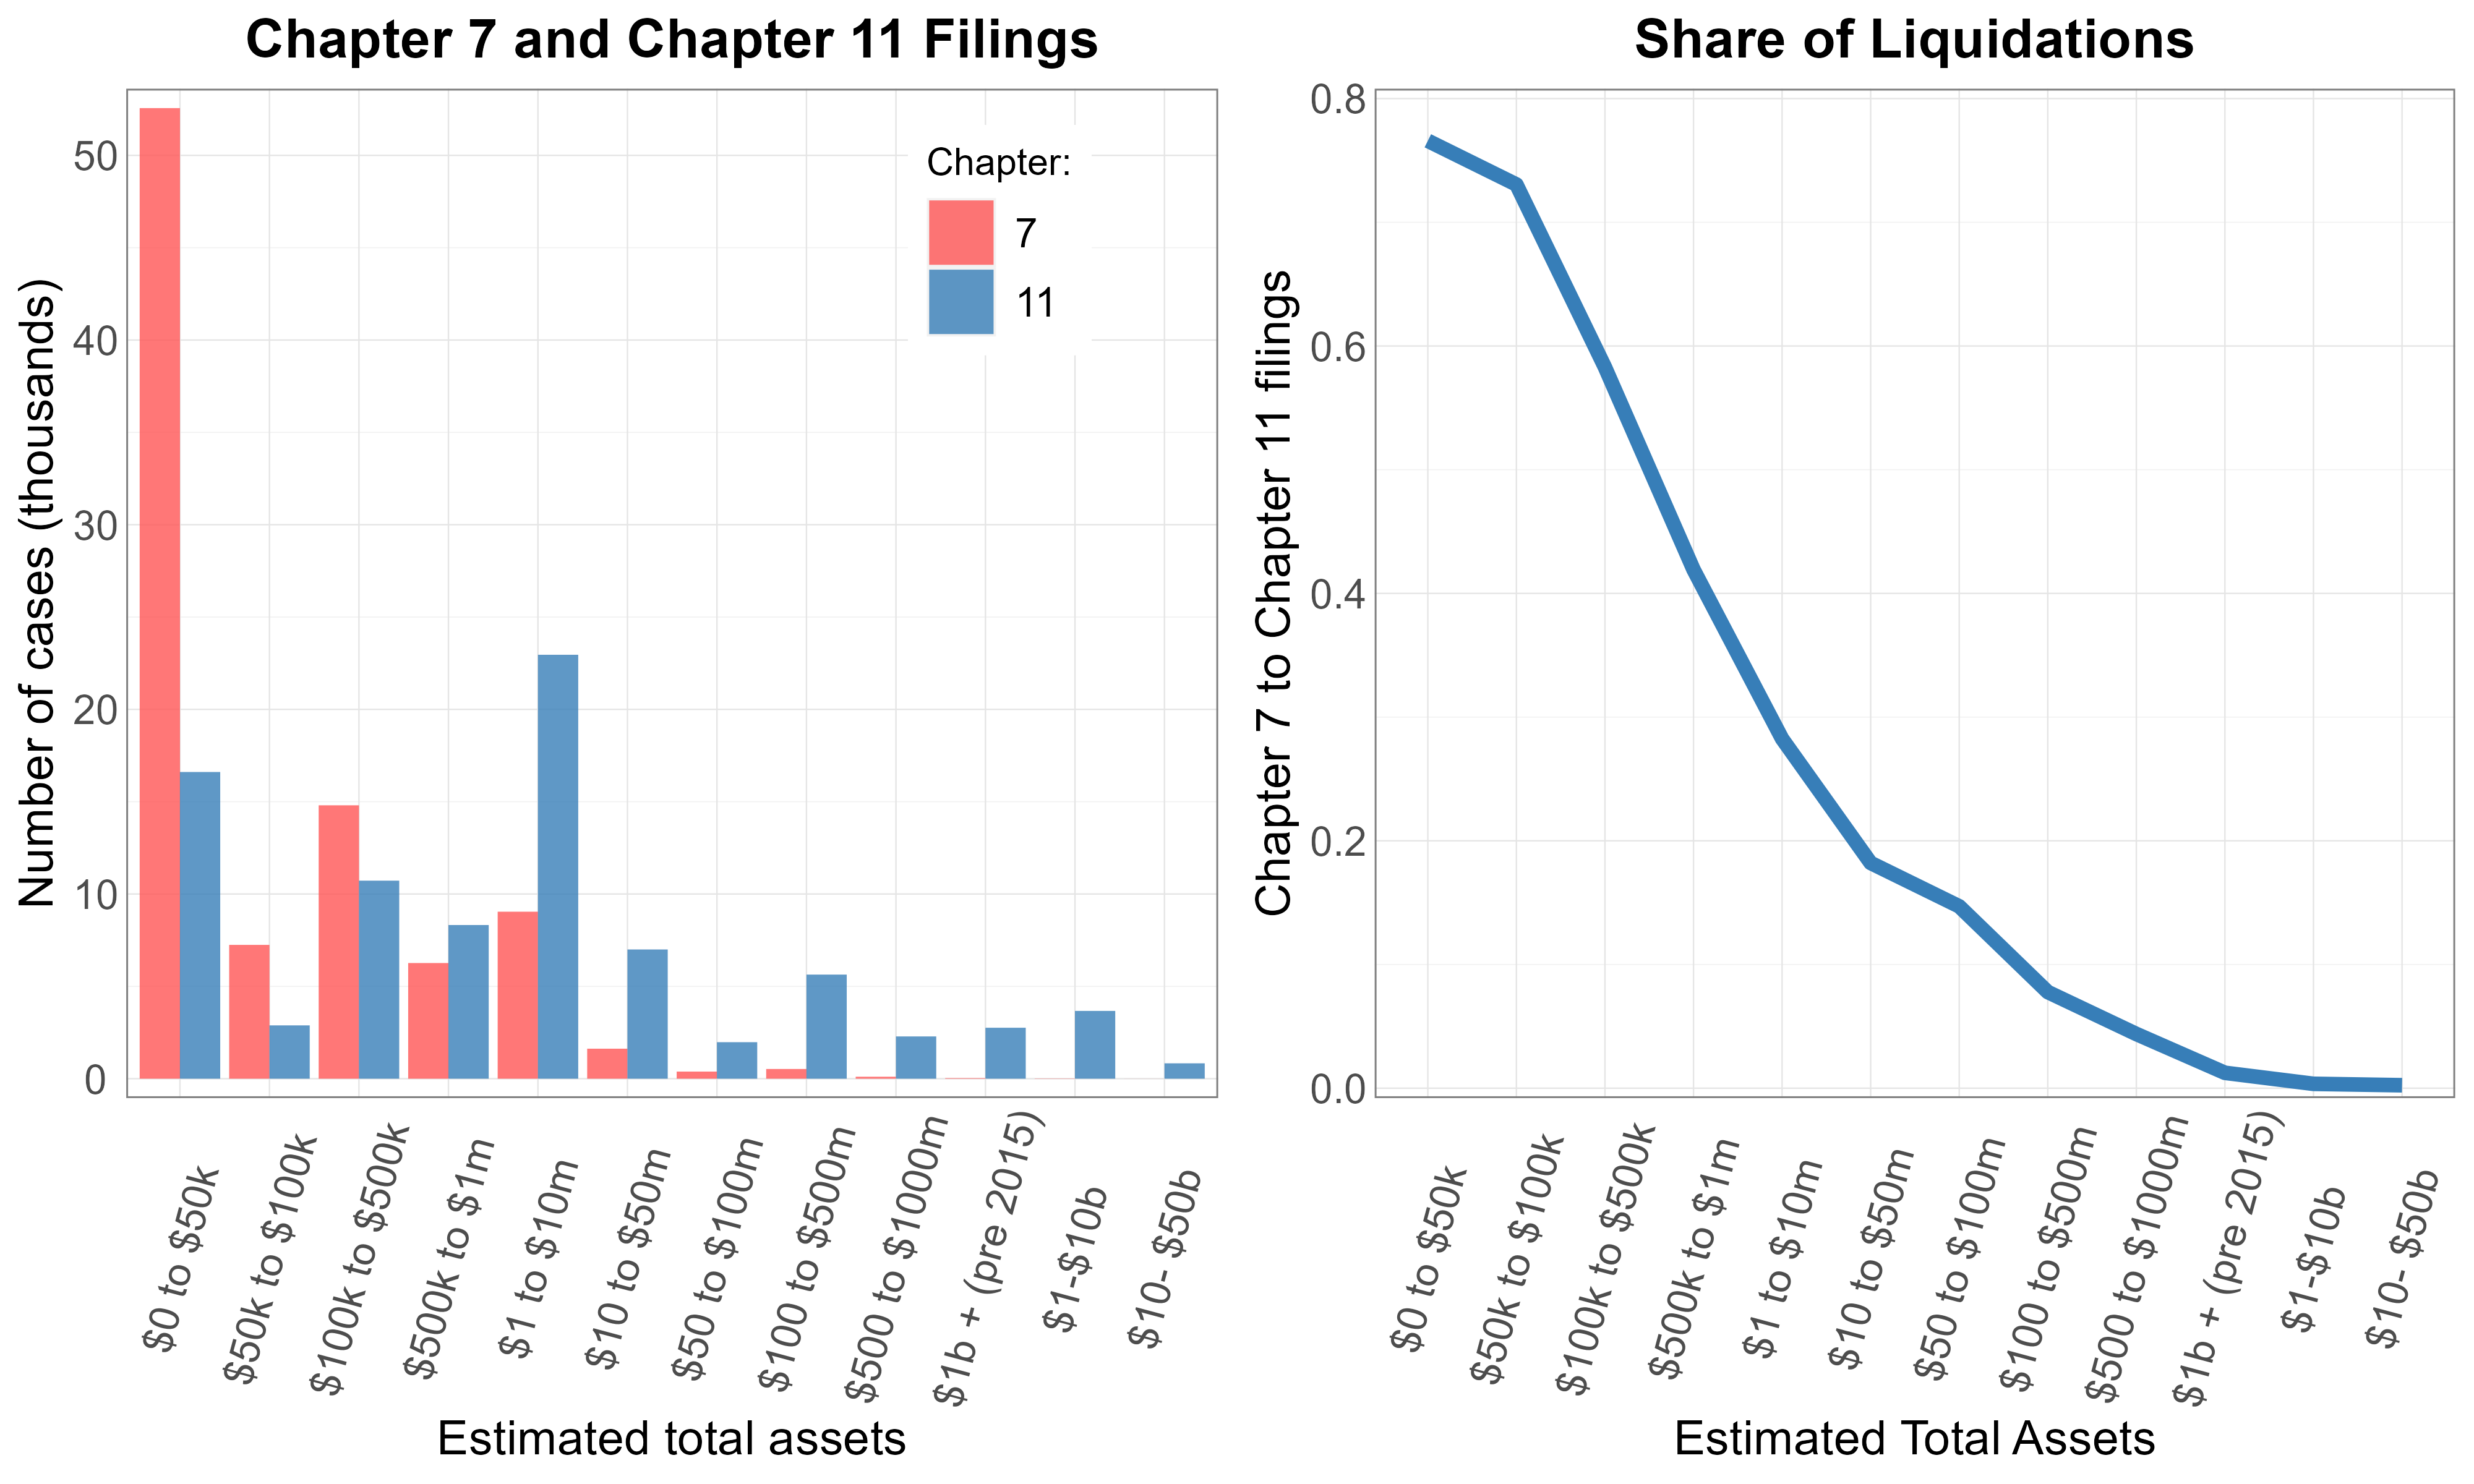
\includegraphics[width=1\textwidth]{C:/Users/szjud/OneDrive/Asztali gép/EBCs/CFL-git/Latex codes/Plots/liqprob2.png}
    \caption{ \small Panel A. shows all Chapter 7 and 11 instances between 2010 and 2023 across firm sizes. Panel B. shows the proportion of Chapter 7 filings as a share of total bankruptcies.}
    \label{chart:liqprob_emp}
\end{figure}

\noindent Resolving default via reorganization often entails lengthy negotiations between debt-ors, creditors and courts, which imposes large time costs as well as administrative and legal expenses on the affected parties. Evidence suggests that a significant share of these costs is independent of firm size. For instance, LoPucki and Doherty (2004, 2011) find that professional fees as a percentage of assets decrease with firm size. Bris et al. (2006) finds similar trend for the total costs of reorganization. The declining probability of liquidation can be attributed to these costs, as small and medium-sized enterprises often lack the resources to cover these expenses. Consistent with these observations, Antill and Grenadier (2018) and Corbae and D'Erasmo (2021) replicate the decreasing liquidation probability in structural models by incorporating large \textit{fixed costs} of reorganization.

\subsection{Credit Spreads and Liquidation Risk \label{sec:emp liqrisk}} 

I study the determinants of credit spreads on a total of 113,774 debt contracts held by 6,925 non-financial corporations between 2010Q1 and 2023Q2.\footnote{Debt-level data is provided by S\&P's Capital IQ and firm-level data is from Compustat North America.} This is a broad, but not representative sample of US non-financial corporations and their debt financing strategies. Section \ref{sec:sumstat} of the appendix presents firm-level firm-level summary statistics. Classification into asset-based and CF-based debt contracts follows the principles outlined by Lian and Ma (2021) - see section \ref{sec:classification} of the appendix. I find that $52.7\%$ of debt contracts can be classified cash flow-based. Since these are often large in terms of value, they collectively constitute 76.7\% of the total debt by volume, which aligns well with the aggregate values reported by Lian and Ma (2021).\footnote{Note however, that my approach is likely to yield a cruder classification, as I have considerably less data at my disposal.}   \vspace{3mm} \\ 
Table \ref{tab:spread_table} summarizes the main determinants of credit spreads for asset-based and CF-based debt contracts as well as the entire sample. Credit spreads are calculated as the difference between interest rates and the treasury rate at the corresponding maturity. To ensure that the observed spread reflects the original contract terms of the loan, I consider debt contracts only at the time of issuance. All three specifications include period fixed effects, sector and credit rating dummies, the logarithm of firm age and employment as well as the share of CF-based debt relative to total debt. Section \ref{sec:credit spreads} of the appendix discusses these factors in more detail and table \ref{tab:spread_table_full} in the appendix presents the full regression output. \vspace{3mm} \\
To test the robustness of my results, I repeat these analyses using interest rates as the dependent variable and at a firm-level, using average credit spread as the dependent variable. These results are reported in \ref{sec:robustness}. 

\begin{table}[H]
    \centering
    \resizebox{\textwidth}{!}{%
    \begin{tabular}{lcccccc}
    \toprule
    & \multicolumn{2}{c}{All contracts} & \multicolumn{2}{c}{CF contracts} & \multicolumn{2}{c}{AB contracts} \\
    \cmidrule(lr){2-3} \cmidrule(lr){4-5} \cmidrule(lr){6-7}
    \textbf{LHS}: Spread & Value & SE & Value & SE & Value & SE \\
    \midrule
    Log of EBITDA & -0.163*** & (0.011) & -0.119*** & (0.012) & -0.205*** & (0.020) \\
    Leverage & 1.759*** & (0.105) & 2.189*** & (0.136) & 0.963*** & (0.176) \\
    Log of Assets & -0.394*** & (0.049) & -0.452*** & (0.060) & -0.321*** & (0.086) \\
    Pledgeability & -0.479*** & (0.087) & -0.046 & (0.107) & -1.013*** & (0.153) \\
    Num. Contracts  & 0.003** & (0.002) & 0.012*** & (0.002) & 0.003 & (0.004) \vspace{3mm} \\
    \midrule 
    Firm-level controls & Yes & & Yes & & Yes & \\
    Period fixed effects & Yes & & Yes & & Yes & \\
    Observations & 17,601 & & 10,620 & & 6,981 & \\
    R-squared & 0.285 & & 0.404 & & 0.174 & \\
    \bottomrule
    \end{tabular}%
    }
    \caption{\small The main determinants of credit spreads of new issuances. Firm level controls include sector and credit rating dummies, the logarithm of firm age and employment, and the share of CF-based debt relative to total debt. Robust standard errors are reported in parentheses, *** p$<$0.01, ** p$<$0.05, * p$<$0.1. The full regression table is reported in section \ref{sec:credit spreads} of the appendix.}
    \label{tab:spread_table}

\end{table}

\noindent 
Lenders perceptions of ex-ante liquidation probability is not directly observable. Therefore, I present \textit{indirect} empirical evidence suggesting that liquidation risk raises credit spreads for CF-based debt contracts. Prior research suggests that higher number of creditors increase the coordination failures in reorganization, thus raising the likelihood that default is eventually resolved by liquidation (Gilson et al., 1990; Brunner and Krahnen, 2008; Zhong, 2021). Applied to CF-based debt financing, these contributions imply that the number of creditors increases spreads on CF-based debt contracts. In contrast, asset-based debt is largely unaffected liquidation risk, hence the number of creditors is expected to have little to no effect on the credit spreads these contracts. \vspace{3mm} \\
This is confirmed by the empirical analysis. The number of debt contracts held by a firm, which is used as a proxy for the number of creditors, is associated with significantly higher spreads on CF-based debt contract - a one standard deviation increase in the number of debt contracts raises credit spreads by 0.168 percentage points. In contrast, this effect is much smaller and statistically insignificant on asset-based debt contracts. Moreover, secured creditors are incentivized to obstruct the reorganization process (Ayotte and Morrison, 2009; Blazy and Choppard, 2010), which amplifies ex-ante liquidation risk further. Consistent with this argument, I find that the number of \textit{secured} debt contracts increases spreads for CF-based debt contracts to an even greater extent - see table \ref{tab:spread_table_new} in the appendix.  \vspace{3mm} \\
The final piece of evidence on the relevance of liquidation risk concerns the relationship between asset pledgeability and credit spreads. Table \ref{tab:spread_table} shows that greater total asset value is associated with lower credit spreads for both loan types.\footnote{Pledgeability is defined as the ratio of collateralizable assets to total assets—see Section \ref{sec:A3} of the Appendix for precise variable definitions.} However, for CF-based debt contracts, asset pledgeability has no significant effect on spreads, suggesting that lenders do not view asset values as a direct determinant of in-default payoffs. Instead, they perceive firm size as a virtue in itself, which may reflect the declining probability of liquidation across firms sizes. Alteratively, this observation could reflect that information asymmetries are typically less severe for large firms.\footnote{For instance, larger firms may follow superior accounting practices, which could mitigate information asymmetries between borrowers and lenders (Zhou, 2007).} To control for the effects of information asymmetries as much as possible, I include firm age and credit rating dummies in the estimation

\section{Model outline} \label{sec:model}
This section introduces a discrete-time general equilibrium model with firms that are heterogeneous in productivity, own capital and may borrow against assets or cash-flows. Firms may experience financial distress, which is resolved either through liquidation or reorganization. Reorganization incurs a fixed costs, making larger firms better positioned to escape liquidation in default. The competitive lender must adjust the terms of the debt contract accounting for credit risk. CF-based debt is not secured by physical collateral, meaning that it exposes the lender to liquidation risk. Finally, the representative household that provide an inelastic labour supply, chooses a stream of consumption and one-period, noncontingent bonds to maximize expected discounted utility. 
\subsection{Heterogenous Firms \label{sec:firms}}
Firms produce a homogeneous consumption good, using labour $n$ and capital $k$, with a decreasing returns to scale production technology:
\begin{equation} \label{eq:prodf}
y = \varepsilon k^{\alpha}n^{\nu}, \ \ \ \ \alpha,\nu \in (0,1),  \ \nu + \alpha \in (0,1)
\end{equation}  
where $\varepsilon$ is the idiosyncratic productivity state. In the interest of keeping the notation simple, I omit firm subscripts. \vspace{3mm} \\
Firms own capital and investments are financed partly by retained earnings and partly by borrowing from a competitive lender. At any given period, a firm can be described by the predetermined capital stock $k \in \mathbf{K} \subset \mathbf{R^{+}}$, debt $b \in \mathbf{B} \subset \mathbf{R}$ and current productivity $\varepsilon \subset \mathbf{R^+}$.  Idiosyncratic productivity is a Markov chain on the finite set $\varepsilon \in \mathbf{E} \equiv \{ \varepsilon_1,...,\varepsilon_{N_{\varepsilon}} \}$ such that $ g_{ij} \equiv \Pr(\varepsilon'= \varepsilon_j|\varepsilon = \varepsilon_i) \geq 0$ and $\sum_{j=1}^{N_{\varepsilon}} g_{ij} = 1$ for each $i$. Moreover, it is stochastically monotone such that for any fixed $x$, $\Pr(\varepsilon' \leq x | \varepsilon = \varepsilon_i)$ is decreasing in $\varepsilon_i$. The distribution of firms can be summarized using the probability measure $\mu$ defined on the Borel algebra $A$, generated by the open subsets of the product spaces $ \mathbf{A} = \mathbf{K} \times \mathbf{B} \times \mathbf{E} $.

\subsubsection{Labour Demand and Production \label{sec:labour demand}}
Production occurs before the realization of exit and entry decisions, and optimal labor demand is independent of current debt. Therefore, at the beginning of the period every firm of state vector $(k,\varepsilon)$ faces the same static optimization with respect to labour: 
$$ \pi(k,\varepsilon) = \max_{n} \ \  \varepsilon k^{\alpha}n^{\nu} - wn - c$$
where $c$ is a fixed cost of participating in production, $w$ is the wage and the price of the consumption good is flexible and normalized to $1$. Optimization yields the policy function for labour demand, $n(\varepsilon,k)$ and optimal production $y(\varepsilon,k)$: 
\begin{equation} \label{eq:opt_emp_prod}
n(k,\varepsilon) = \left( \dfrac{ \nu \varepsilon k^\alpha}{w} \right)^{\frac{1}{1-\nu}} \hspace{15mm}
y(k,\varepsilon) = \varepsilon k^{\alpha} \left( \dfrac{\nu \varepsilon k^\alpha}{w} \right)^{\frac{\nu}{1-\nu}}.
\end{equation}  
Firm profit function can be reformulated as: 
\begin{equation} \label{eq:profit}
\pi(k,\varepsilon) = y(k,\varepsilon) - wn(k,\varepsilon) - c = (1-\nu) y(k,\varepsilon) - c.
\end{equation} 
Firms own capital and make investment decisions, subject to a capital accumulation function,
\begin{equation} \label{eq:capital}
k' = (1-\delta)k + i
\end{equation} 
where $\delta$ is the depreciation rate and $i$ is investment. Since capital and debt are free of adjustment costs, the financial position of firms can be summarized by the cash on hand variable:
\begin{equation} \label{eq:cash on hand}
    x = \pi(k,\varepsilon) + (1-\delta)k - b.
\end{equation}

\subsubsection{Firm Values} \label{sec:Firm Values}
Production takes place at the beginning of the period. Firms set their labour demand given $(k,\varepsilon)$, profits are realized and capital depreciates. Then, incumbents may decide to exit, default or continue production to the next period. This decision is governed by: 
\begin{equation} \label{eq:default decision}
    V_0(k,b,\varepsilon) = \max \{V_{def}, \  V_{exit}(k,b,\varepsilon),  \ V_{cont}(k,b,\varepsilon) \}.
\end{equation}
Default is associated with zero value independent of the default resolution, such that reorganization costs only affect firm values through their effects on credit market conditions,\footnote{Jostarndt and Sautner (2008) and Ayotte and Morrison (2009) find that the management of the firm is typically replaced under the reorganization process, meaning that this assumption could be interpreted as the management being indifferent between reorganization and liquidation after default occurs.} 
\begin{equation}
    V_{def} = 0.
\end{equation}
Firms may also decide to exit after repaying their debt obligations. This allows firms to retain the value of the undepreciated capital stock net of debt service: 
\begin{equation}
    V_{exit}(k, b, \varepsilon) = \pi(k,\varepsilon) + (1-\delta)k - b  = x.
\end{equation}
Firms that decide to continue can obtain external financing through one-period debt contracts. For each unit of debt due in the next period, they receive $q$ units of output, which can be used towards investment or distributed as dividends. Moreover, continuing firms decide what proportion of their debt to be backed by future cash flows. In the following, I refer to this as the debt financing strategy of the firm and it is summarized by $\tau \in [0,1]$, where $\tau$ measures the value of CF-based to total debt - analogously to the `CF-share' introduced in the empirical analysis. \vspace{3mm} \\
Continuing firms choose future capital stock $k'$, total future debt $b'$, and debt financing strategy $\tau'$ to maximize the discounted sum of dividends $d$, 
\begin{equation} \label{eq:dividends}
d = x - k' +  q(k',b',\varepsilon, \tau')b'.
\end{equation} 
Since capital and debt are not subject to adjustment costs, firms' financial position can be summarized by the cash on hand variable defined in equation \ref{eq:cash on hand}. This reformulation is reduces the computational burden of the model. Using the cash on hand variable, the value of continuation can be described as,
\begin{equation} \label{eq:V_cont}
    V_{cont}(x,\varepsilon) = \max_{k',b', \tau'} \left(x - k' +  q(k',b',\varepsilon, \tau')b' + q_f \E_{\varepsilon'|\varepsilon} V(k',b', \varepsilon') \right)
\end{equation}
subject to: 
\begin{equation} \label{eq:budget}
x' = \pi(k',\varepsilon')+(1-\delta)k'-b' \hspace{5mm} \text{and} \hspace{5mm} d \geq 0
\end{equation} 
where $q_f$ is firms' subjective discount factor. Note that since firms are owned by the household, future dividend payments are discounted using the household's discount factor, $\beta = q_f$. In the following, I summarize the collection of decision variables as $a = (k, b, \tau) $, section \ref{sec: Financial Intermediation} describes how the inverse interest rate depends on these decision variables.  \vspace{3mm} \\
Finally, entrants are endowed with zero starting cash on hand, reflecting that startups are typically asset-poor. These firms do not produce in the first period, and have the option to exit after drawing an initial productivity value. Hence, their initial decision can be described as: 
\begin{equation} \label{eq:entrant decision}
    V_e(\varepsilon) = \max \{0,  \ V_{cont}(0,\varepsilon) \}.
\end{equation}
That is, potential entrants solve \ref{eq:V_cont} - \ref{eq:budget} similarly to continuing firms, with the difference that their cash on hand is exactly zero. If $V_{cont}(0,\varepsilon)$ is smaller than zero, they exit voluntarily, without ever participating in production.

\subsubsection{Firm dynamics}
To describe firm dynamics, I define the following indicator function. Let $\chi_{d} = 1$ if the firm defaults either due to endogenous decisions or the exogenous shock, $\chi_l = 1$ if the firm is liquidated in default (this decision is further discussed in section \ref{sec:default resolution})  and let $\chi_{ex} = 1$ if the firm exits voluntarily, after fulfilling its debt obligations. \vspace{3mm} \\
Voluntary exits and liquidations are balanced by a mass $M$ of potential entrants. Entrants' initial productivity is drawn from the stationary distribution of the Markov chain that defines idiosyncratic productivity - this is denoted by $\Phi(\varepsilon)$. Let $\mu_0$ be the measure of the mass of firms at the beginning of the period. Then, taking stock movements on the extensive margin, the measure of firms at the end of the period can be expressed as: $\mu = (1 - \chi_l - \chi_{ex}) \mu_0  + (1 - \chi_{ex}) M d \Phi(\varepsilon) $. \vspace{3mm} \\
The evolution of firm distribution satisfies: 
\begin{equation} \label{eq_firmdim} 
    \mu_{0}'(A) = \int \mathbf{I}_{(k', b', \varepsilon') \in A} g(\varepsilon'|\varepsilon) \ d \mu (k,b,\varepsilon)
\end{equation}
for all Borel sets $A \subset  \mathbf{K} \times \mathbf{B} \times \mathbf{E} $ and where $g(\varepsilon'|\varepsilon)$ is the transition probability matrix idiosyncratic productivity. Finally, I summarize the dynamics of firm distribution at the beginning of the period by the mapping $ \mu'_0 =\Gamma(\mu_0)$.


\subsection{Financial Intermediation}  \label{sec: Financial Intermediation}
\subsubsection{The lender's problem}    \label{sec: The lender's problem}
The opportunity cost of lending to firms is determined by the risk-free bond yield $q_0$. However, since corporate lending is subject to default risk, the competitive lender must charge a premium to break even. When setting $q(a',\varepsilon)$ the lender must consider the expected payoff under 3 distinct scenarios: \textit{a)} orderly repayment; \textit{b)} the firm defaults and is liquidated \textit{c)} the firm defaults and is reorganized. It follows from the zero-profit condition that the debt schedule offered to firms is, 
\begin{equation} \label{eq:q}
    \begin{split}
        & q(a', \varepsilon)b' = q_0 \left[ \left(1-P_D(a', \varepsilon)\right)b' + \right. \\
        & \qquad P_D(a', \varepsilon) \gamma(a', \varepsilon) \min \{b', \ \Pi_{l}(a')\} + \\ 
        & \qquad \left. P_D(a', \varepsilon) (1-\gamma(a', \varepsilon))\min \{b', \ E_{\varepsilon' | \varepsilon} [ \Pi_{r}(a', \varepsilon') |\chi_r = 1 ] \} \right]
    \end{split}
\end{equation}
where 
\begin{itemize}\setlength\itemsep{0em} 
    \item $\Pi_{l}(a')$ is the expected payoff if the firms undergoes liquidation,
    \item $\Pi_{r}(a', \varepsilon)$ is the expected payoff if the firms undergoes reorganization,
    \item $P_D(a', \varepsilon)$ is the probability of default,
    \item $\gamma(a', \varepsilon)$ is the probability of liquidation under financial distress. 
\end{itemize} 
In the following, I discuss the determinants of these values. This yields a complete description of the debt schedule $q(a', \varepsilon)$.


\subsubsection{Default and Default Resolution} \label{sec:default resolution}
Firms may default endogenously, following decision rule specified in equation \ref{eq:default decision}. Additionally, they may experience an exogenous default shock, which reaches all firms with a uniform probability $P_{x}$ - this shock is necessary to calibrate the share of reorganizations to the data. The ex-ante probability of default can be described as: 
\begin{equation} \label{eq:default probability}
    P_D(a', \varepsilon) = E_{\varepsilon'|\varepsilon}[\chi_{endo}(a',\varepsilon')] + P_{x} - E_{\varepsilon'|\varepsilon}[\chi_{endo}(a',\varepsilon')]P_{x}
\end{equation}
where $\chi_{endo}(x, \varepsilon) = 1$ if the firms defaults endogenously. \vspace{3mm} \\ 
Defaults can be resolved through liquidation or reorganization. In the case of liquidation, the firm exits, and all its undepreciated capital stock is resold at a discounted value, $\phi_l(1-\delta)k$, where $\phi_l \in (0,1)$. The rest of the stock cannot be recovered, which indicates that corporate assets are often highly specialized and illiquid (Kermani and Ma, 2020). The proceeds from selling the capital stock are distributed between the lender and the household. The exact allocation depends on the debt contract in place, this is further discussed in following section. \vspace{3mm} \\
Reorganization allows the firm to continue, but it incurs a variable $\phi_r V_{cont}(x,\varepsilon)$ and a fixed cost $\zeta_r$ as well, which are borne by the household.\footnote{The incidence of these cost has a minimal effect credit market frictions. Lenders' expenses directly raise the external finance premium, whereas households' costs limit access to external finance indirectly by raising liquidation risk.} This fixed cost introduces economies of scale into the reorganization process, hence it crucial in replicating the decreasing liquidation probability in the function of firm size - I discuss the sources of these costs in section \ref{sec:fixed costs} of the appendix. Moreover, the household pays a fraction of the firms' continuation value to the lender as a lump-sum transfer. This represents the renegotiation of the debt contract.\footnote{Corbae and D'Erasmo also model the reorganization process as a lump-sum transfer between the lender and the borrower. However, their approach is richer, as they model the Nash Bargaining process that determines the value of the transfer.} The exact value of this transfer depends on the debt contract in place, and it is further discussed in the following section. \vspace{3mm} \\
To keep the model parsimonious, I assume that default resolution decision maximizes the value retained after bankruptcy, and does not consider the allocation of payoffs between the lender and the household. Hence, the default resolution decision can be summarized as: 
\begin{equation} \label{eq:liquidation decision}
    \max \{ \phi_l (1-\delta) k; \ (1-\phi_r) V_{cont}(x,\varepsilon)- \zeta_r  \}
\end{equation}
And the ex-ante probability of liquidation under financial distress can be defined as: 
\begin{equation} \label{eq:liquidation probability}
    \gamma(a', \varepsilon) = Pr(\phi_l (1-\delta) k \ \geq \ (1-\phi_r) V_{cont}(x,\varepsilon) - \zeta_r | \chi_d = 1)
\end{equation} 
This highly stylized description of the default resolution process, is sufficient for the purposes of this discussion as it captures the decreasing liquidation probability across firm sizes. In practice, the default resolution process typically involves negotiations between the borrower and multiple creditors, under the oversight of courts. For more realistic depictions of the bankruptcy process, see Tamayo (2017) and Hu and We (2018).  

 
\subsubsection{Lenders' In-default Payoffs}   \label{sec:Default Payoffs}
This section describes lenders' in-default pay-offs depending on the default resolution and the debt contract in place. These pay-offs are central to the analysis as they shape the debt schedule $q(a', \varepsilon)$, that firms must consider in choosing debt financing strategy. The model considers two loan-types (asset-based and cash flow-based) and two bankruptcy types (liquidation and reorganization), therefore the lender has four distinct cases to consider. \vspace{3mm} \\
\textit{ 1.) The recovery of asset-based debt when the firm undergoes liquidation}. Since the debt contract is backed by physical assets, the lender can recover the entire liquidation value of the firm, $\phi_l(1-\delta)k$. Note that this case corresponds to the traditional assumption on lenders' in-default payoffs when only asset-based debt is available.  \vspace{3mm} \\
\textit{ 2.) The recovery of asset-based debt when the firm undergoes reorganization}. When the borrower undergoes reorganization secured lenders are protected by the ‘best interest of creditor’ test.\footnote{The EU Directive refers this principle as ‘best-interest-of-creditors’ test in OJ L 172/27, art. 49; whereas the US bankruptcy code establishes this principle in - see section \ref{sec:A1} in the appendix} This states that creditors cannot be worse off under the proposed reorganization plan than they would be under liquidation. Accordingly, I assume that the lender can retrieve the same $\phi_l(1-\delta)k$ as they would do under liquidation. \vspace{3mm} \\
\textit{ 3.) The recovery of CF-based debt when the firm undergoes liquidation}. In this case, the debt is not backed by physical collateral, which makes the lender ill-equipped to recover the liquidation value.  As a result, the lender can only recover a small fraction of the total liquidation value, $\kappa \phi_l(1-\delta)k$, where $\kappa$ is close to zero. \vspace{3mm} \\
\textit{ 4.) The recovery of CF-based debt if the firm undergoes reorganization}. In this case, the lender can claim a fraction of the continuation value such that its payoff is $\phi_c V_{cont}(x,\varepsilon)$. Hence, in this case the lender's payoff is determined by the continuation value of the firm - for an analogous description of lenders in-default payoffs after CF-based debt, see Drechsel (2023). In practice, this process may vary depending on specifics of the debt contract. When the debt is secured against the entire corporate entity, the lender may gain access to borrower's cash flows directly. When the debt is unsecured, higher continuation value of the firm allows the lender to negotiate better terms during reorganization - for a detailed description of this mechanism see Corbae and D'Erasmo (2021). \vspace{3mm} \\
These four payoffs above summarize the trade-offs between lending against future cash flows and physical assets. It is now possible to outline the lender's expected payoff depending on debt financing strategy adopted prior to bankruptcy. Recall that the share of CF-debt to total debt is defined by $\tau \in (0,1)$. Hence, the lender's payoff under liquidation (or reorganization) is a linear combination of the payoffs from asset-backed debt (with weight $\tau$) and CF-debt (with weight $1-\tau$). \vspace{3mm} \\
First, consider debt-recovery under liquidation. The total value available after the liquidation of firms' assets is $\phi_l (1-\delta) k$. However, the lender can only retrieve this value for the debt that is backed by physical assets, which is $1-\tau$ share of the total debt. After the remaining $\tau$ share, which corresponds to CF-based debt, the lender can seize only $\kappa$ fraction of original value. Whatever is not seized by the lender under the default resolution is redistributed to the household as a lump sump transfer. Taking stock, the if the borrower is liquidated the lender receives,
\begin{equation} \label{eq:P_liq} 
   \Pi_{l}(a) = (1-\tau) \phi_l (1-\delta) k +\tau \kappa \phi_l  (1-\delta) k. 
\end{equation}
When the firm undergoes reorganization the lender can claim a fraction of future cash flows after CF-based debt. Moreover, in accordance with the `best interest of creditor test' the lender to retrieve a payment that is equal to the liquidation value of the collateral after asset-based debt. Hence, under reorganization the lender receives,
\begin{equation}  \label{eq:P_reorg}
   \Pi_{r}(a,\tau) = (1-\tau) \phi_l (1-\delta) k +\tau \phi_c V_{cont} (x, \varepsilon).
\end{equation}
This concludes the description of the four values that lenders must consider when lending against assets or future cash-flows. These are, default probability (equation \ref{eq:default probability}), liquidation probability (equation \ref{eq:liquidation probability}), and expected payoff under liquidation and reorganization (equation \ref{eq:P_liq} and \ref{eq:P_reorg} respectively). Together with equation \ref{eq:q}, these yield a complete description of the debt schedule $q(a', \varepsilon)$ that continuing firms must consider. 

\subsection{Households}\label{sec:hh}
\subsubsection{Consumption and Savings Decision} \label{sec:Cons and Savings decision}
There is a unit measure of identical households that choose a stream of consumption $C$ and one-period, noncontingent bonds $B$ which yield the risk free interest rate $q_0$ to maximize expected discounted utility. Households take firm measure $\mu_0$ as given. Their problem can be defined recursively as: 
\begin{equation} \label{eq:U_max}
V_h(B, \mu_0) = \max_{C,B'} U(C) + \beta V_h(B',\mu_0')
\end{equation}  
subject to: 
\begin{equation} \label{eq:const_hh}
C + B \leq w N^s + q_0 B' + T
\end{equation} 
where $N^s$ is the inelastic labour supply, $\beta$ is the households' discount factor and $T$ denotes expenses and revenues from the production sector, shared within the household. Revenues include dividends from continuing firms and net wealth from exiting firms and the value not seized by the lender after liquidations. Expenses cover the the costs of reorganization, and transfers to the lender under the debt renegotiation process:
\begin{equation*} \label{eq:T}
    \begin{split}
        & T = \int (1 - \chi_l - \chi_{ex}) \left( x - k'(k,b,\varepsilon) + qb'(k,b,\varepsilon) \right) d \mu_0(k,b,\varepsilon) \\
        & \qquad + \int \chi_{ex} \ x \ d \mu_0(k,b,\varepsilon) \\
        & \qquad + \int \chi_d \chi_{l} [ \phi_l (1-\delta) k -  \min\{b, (1-\tau) \phi_l (1-\delta) k +\tau \kappa \phi_l  (1-\delta) k \} ] \ d \mu_0(k,b,\varepsilon)  \\
        & \qquad  - \int \chi_d (1-\chi_{l}) \ \min\{b, (1-\tau) \phi_l (1-\delta) k +\tau \phi_c V_{cont} (x, \varepsilon)        \} \ d \mu_0(k,b,\varepsilon) \\
        & \qquad  - \int \chi_d (1-\chi_{l}) \  [ \phi_r V_{cont} (x, \varepsilon) + \zeta_r] \ d \mu_0(k,b,\varepsilon).
    \end{split}
\end{equation*}

\subsection{Stationary equilibrium}\label{sec:eq}
The stationary competitive equilibrium is described by the set of functions
$$(\mu_0, \mu, w, V, V_{cont}, V_{def},  V_{exit}, V_r, V_r, \chi_l, \chi_l, \chi_{ex}, n,k,b,d,\tau,q, C, B)$$
such that: 
\begin{enumerate}[(i)]
\item households solve utility maximization: $V_h$ solves \ref{eq:U_max}-\ref{eq:const_hh} and the associated policy functions are $(C, B)$;
\item the lender solves \ref{eq:q} such that $q(a',\varepsilon)$ yields zero profits in expectation on each debt contract;
\item firms solve value maximization: $V_0$ solves \ref{eq:default decision} and $V_{cont}$ solves \ref{eq:profit}, \ref{eq:V_cont} and \ref{eq:budget}; and the associated policy functions are $n$, for exiting and defaulting firms and $(n,k,b,d,\tau,q)$ for continuing and entering firms;
\item the default resolution solves \ref{eq:liquidation decision} 
\item wages adjust to equate firms' labour demand to the inelastic labour supply
$$ N^s = \int n  \ d \mu_0 (k,b,\varepsilon)  $$
\item the first order condition households' savings problem implies that the interest rate of the noncontingent bond $q_0$ is equal to households' discount parameter $\beta$; and the financial market clears at $q_0 = q_f = \beta$
 $$ B = \int b \ d \mu_0 (k,b,\varepsilon) $$
\item goods market clears due to Walras' law (binding budget constraints and all other markets are in equilibrium) and aggregate consumption is
 $$ C = Y - I - \Psi$$
where
 $$ Y =  \int y \ d \mu_0 (k,b,\varepsilon) $$
aggregate investment is the sum of investment carried out by continuing incumbents and entering firms minus the capital freed up due to liquidations and voluntary exits:
\begin{multline*} 
    I = \int   k' -(1-\delta)k \ d \mu (k,b,\varepsilon) + M \int (1-\chi_{ex}) k' \ d \Phi(\varepsilon)    \\
   -  \int   \chi_l \chi_d \phi_l (1-\delta)k \ d \mu_0 (k,b,\varepsilon) - \int \chi_{ex} (1-\delta) k \ d \mu_0 (k,b,\varepsilon)   
\end{multline*}
$\Psi$ collects the fixed costs of operation and the costs of default resolution:
\begin{multline*} 
    \Psi = \int  \chi_l \chi_d (1-\phi_l) (1-\delta)k \ d \mu_0 (k,b,\varepsilon)  \\ + \int  (1 - \chi_l)  \chi_d [\phi_r V_{cont}(x, \varepsilon) + \zeta_r] \ d \mu_0 (k,b,\varepsilon) + \int  c \ d \mu_0 (k,b,\varepsilon) 
\end{multline*}
\item the distribution measure of firms is stationary, $\Gamma(\mu_0) = \mu_0$ and prices $(w,q)$ are constant over time.
\end{enumerate}


\section{Calibration and Model Fit}
I calibrate the model at a yearly frequency. The first set of parameters are set externally, based on comparable structural models, common values adopted in the literature and previous empirical results. Decreasing returns to scale parameter is set $DRS = 0.75$, the capital share of production is $\alpha$ is one-third and the labour share is $\nu$ is two-thirds. The subjective discount parameter of the household is $\beta = 0.96$ and depreciation is $\delta = 0.1$. These parameter parameter values are within the range of standard values adopted in the literature. The resale value of assets is, $\phi_l = 0.4$ calibrated based on Kermani and Ma (2020), who estimates the average recovery rate of assets after liquidation. If the debt is not secured by physical assets, the lender can only seize $\kappa = 0.1$ share of this value - since this variable has minimal impact on the steady state, it is not calibrated separately. \vspace{3mm} \\
The productivity process is based on Di Nola, Kaas and Wang (2023). Idiosyncratic firm productivity follows the AR(1) process 
$$ \ln(\varepsilon_{t+1}) = (1-\rho) \ln(\varepsilon_0) + \rho \ln(\varepsilon_t) + \sigma \zeta_\varepsilon, $$ where 
$\rho = 0.969$ is the persistence of productivity the shock, $\varepsilon_0 = 1$ is the normalized average productivity and $\sigma = 0.146$ is the standard deviation of idiosyncratic productivity shocks.  The log-process is discretized using Tauchen's method.  \vspace{3mm} \\
I calibrate the rest of the model parameters using a combined dataset of CapitalIQ, Compustat and Federal Judicial Center's Integrated Database (IDB). This presents a challenge, as smaller firms are underrepresented in Compustat-CapitalIQ and likely to be overrepresented in the IDB. To align these two datasets, I classify firms into two categorizes: small firms, with less than 10 million in liabilities and large firms than 10 million in liabilities.\footnote{This cutoff corresponds the largest firm category (by total liabilities) that could be covered by the SBRA.} In Compustat, small firms add up to around 21\% of the sample, whereas in IDB these firms are 67\% of the sample.\footnote{I do not consider `micro' firms that have less than 100k USD of total assets, as they are not represented in the Compustat.} The targeted moments are calculated by mapping Compustat values onto the IDB firm distribution.

\begin{table}[h!]
    \centering
    \begin{tabular}{c|c|c}
    \multicolumn{3}{l}{\textbf{Externally Calibrated Parameters}} \\ 
    \midrule
    DRS & Decreasing returns & 0.75 \\
    $\alpha$ & Capital Share of Output & 0.33 \\
    $\beta$ & Discount Rate & 0.96 \\
    $\delta$ & Depreciation rate & 0.1 \\
    $\rho$ & Produ . Shock Persistence & 0.969 \\
    $\sigma_{\varepsilon}$ & Produ . Shock SD & 0.146 \\
    $\varepsilon_0$ & Average Productivity & 1 \\
    $\phi_l$ & Resale value of assets & 0.4 \\
    $\kappa$ & Unsecured discount & 0.1 \vspace{3mm} \\
    \multicolumn{3}{l}{\textbf{Internally Calibrated Parameters}} \\ 
    \midrule
    $\phi_r$ & Variable cost of reorganization & 0.204 \\
    $\zeta_r$ & Fixed costs of reorganization & 2590 \\
    $ \phi_c $ & Lender's payoff under reorganization  & 0.281 \\
    $P_x$ & Exogenous probability of default & 0.025 \\
    $ c $ & Fixed costs of operation & 30.2 \\
    \bottomrule
    \end{tabular}
    \caption{Externally and Internally calibrated parameters values}
    \label{tab:external calib}
\end{table}

\noindent The internally calibrated parameters are set to match facts about firms' debt financing strategies and default resolution decisions. Due to general equilibrium effects, parameter values cannot be set in isolation. Yet, they can be associated with closely related data moments. Fixed and variable costs of reorganization are set based on the average liquidation probability. Moreover, the fixed cost of reorganization is important in matching the decreasing liquidation probability across firms sizes. On the targeted data moments, this is reflected by the difference between the CFL reliance and the share of outstanding CF-based debt to total debt. The former is significantly lower than the latter because large firms' face minimal liquidation risk and typically borrow against cash flows. Average interest rate is matched by the probability of exogenous default and the debt to collateral ratio is linked to the fixed cost of operation through average firms size. 

\begin{table}[h!]
    \centering
    \begin{tabular}{c|c|c}
    \toprule
    \textbf{SS value} & \textbf{Target value} & \textbf{Model value} \\ 
    \midrule
    Debt to Collateral & 0.49 & 0.47 \\ 
    Average interest rate & 5.3 & 5.37 \\ 
    Average Liquidation prob. & 0.48 & 0.51 \\ 
    Average CF-reliance & 0.43 & 0.49 \\ 
   CF-based to total debt & 0.76 & 0.76 \\ 
    \bottomrule
    \end{tabular}
    \caption{Targeted data moments and their model counterparts}
    \label{tab:targets}
\end{table}

\noindent The targeted moments and their corresponding model values are summarized in table \ref{tab:targets}. The model closely replicates the central facts about firms' debt financing strategy, default resolution decisions as well as the external finance premia they face. To further assess model performance, I compare untargeted moments to their data equivalents. I divide the sample into small and large firms, based on total borrowing. Small firms account for the bottom 66\% of firm distribution, which corresponds to the share of firms in IDB with liabilities under 10 million USD. Table \ref{tab:untargeted}. presents the targeted moments and their corresponding model values separately, for small and large firms.\vspace{3mm} \\
\noindent The model closely replicates the SME financing gap observed in the data. Small firms realize significantly lower debt to collateral ratio while facing higher external finance premia. The decreasing probability of liquidation across firm size is also captured well in the model, although this decline somewhat less pronounced in the data. On the other hand, the model falls short in matching the average CF-reliance. The CFL reliance is in fact U-shaped across firms, with the largest and the smallest firms borrowing most heavily against cash flow (Gonzalez and Sy, 2024). This imprecision arises because the model misses the left side of this U-shape, as it almost always assigns a liquidation probability near 1 to small firms. The ratio of CF-based debt to total debt value is again replicated closely by the model. 

\begin{table}[h!]
    \centering
    \begin{tabular}{c|c|c||c|c}
    \textbf{SS Value} &  \multicolumn{2}{c}{\textbf{Data}} & \multicolumn{2}{c}{\textbf{Model}} \\ 
    \toprule
     & Small Firms & Large Firms & Small Firms & Large Firms  \\ 
    \midrule
    Number share & 0.67 & 0.33 & 0.64 & 0.36 \\ 
    Debt to Collateral & 0.42 & 0.59 & 0.41 & 0.54 \\ 
    Interest Rate (\%) & 5.89 & 4.63 & 5.83 & 4.84 \\ 
    Liquidation Probability & 0.70 & 0.32 & 0.80 & 0.16 \\ 
    CF Reliance & 0.40 & 0.47 & 0.13 & 0.94 \\ 
    CF-based to total debt & 0.32 & 0.77 & 0.25 & 0.80 \\ 
    \bottomrule
    \end{tabular}
    \caption{Untargeted data moments and their model counterparts}
    \label{tab:untargeted}
\end{table}


\section{Results and Discussion \label{sec:results}}

This section presents the main findings of the structural analysis. First, I examine the effects of a policy reform that lowers reorganization costs, significantly reducing liquidation risk. This reform improves access to CF-based debt financing, increasing the mass of active firms and improving credit allocation, which ultimately boosts aggregate productivity. Next, I assess the reform’s impact under alternative model specifications where only asset-based or CF-based lending is available. When asset-based debt is absent the effects of the reform are over-estimated. When CF-based debt contracts are absent, liquidation risk has no influence on financing conditions, which may explain why much of the literature overlooks the importance of high reorganization costs. 

\subsection{The Effects of Reorganization Costs}
In this section, I use the calibrated model as a laboratory to explore the effects of a policy reform that implements a more reorganization-friendly bankruptcy framework. In particular, I study an alternative model calibration in which the fixed cost of reorganization is half of the baseline value, while the variable costs remains unaffected. This represents a large intervention as average liquidation probability falls from 50\% in the baseline model to 32\% after the reform. Moreover, to see how the reform effects would scale, I also consider the effects of an `extreme reform', which reduces the fixed costs of reorganization to one-tenth of the baseline value, limiting average liquidation probability to just 8\%.  The general equilibrium effects of these reforms are summarized in table \ref{tab:SSvalues}. \vspace{3mm} \\ 
Since large firms are relatively unaffected by the fixed cost due to their scale, the reform has the most substantial impact on small firms. Liquidation probability for small firms drops from 0.80 in the baseline calibration to just 0.57 after the reform, which fundamentally changes their debt financing strategy. Smail firms' average reliance on CF-based debt jumps from just 14\% to 50\% and the share of CF-based to total debt volume increases from 25\% to 82\%. Better access to CF-based debt, allows these firms to rely on external finance more intensively. The debt to collateral ratio increases by 4 percentage points, while the average interest rate declines by 0.65 percentage points. These effects point to the same direction for large firms, but are significantly smaller. As a result, the financing gap between small and large firms observed in the baseline calibration narrows considerably after the reform.  \vspace{3mm} \\ 
Average productivity increases by 1.4\% after the reform, reflecting large changes in firms' access to CF-based debt. The total mass of firms increases, while the firm size (measured by labour demand) falls by 4.03\%. Since the production technology is decreasing returns to scale, the fall in average size boosts aggregate productivity. Capital deepening is not substantial, the capital to labour ratio increases only by 0.36\%. Two conflicting forces contribute to this change. When firms borrow against assets, capital serves both as collateral and a productive asset. Hence, when borrowing against cash flows is limited, firms tend to invest more than optimal (Drecshel and Kim, 2022). On the one hand, cheaper access to debt finance allows firms to reach their optimal size faster, which implies larger stock of total capital. Hence, the effect of CF-based debt financing on the capital stock is ambiguous.

\begin{table}[h!]
    \centering
    \begin{tabular}{lccc}
    & \textbf{Baseline} & \textbf{Reform} & \textbf{Extreme Reform} \\    
    \toprule
    \multicolumn{1}{c}{FC of reorganization, $\zeta_{r}$} & 2590 & 1295 & 259  \vspace{3mm} \\  
    \multicolumn{4}{l}{\textbf{Aggregates}} \\ \hline
    Total mass & 13.89 & 14.47 & 14.92  \\
    Mean Employees & 720 & 691 & 670  \\
    Small Firms Share  & 0.64 & 0.64 & 0.64  \\
    Wage & 1.00 & 1.014 & 1.029  \\
    Capital Intensity (K/L) & 2.74 & 2.75 & 2.83  \\
    Productivity (Y/L) & 2.00 & 2.027 & 2.057  \vspace{3mm} \\  
    \multicolumn{4}{l}{\textbf{Bankruptcy Resolution}} \\ \hline
    Pr. Liquidation - Small Firms & 0.80 & 0.57 & 0.15  \\
    Pr. Liquidation - Large Firms & 0.16 & 0.03 & 0.00  \vspace{3mm} \\  
    \multicolumn{4}{l}{\textbf{Debt Financing Strategy}} \\ \hline
    CF reliance - Small Firms & 0.14 & 0.50 & 0.83  \\
    CF reliance - Large Firms & 0.94 & 0.97 & 0.97  \vspace{1mm} \\  
    CF to total debt - Small Firms & 0.25 & 0.82 & 0.97  \\
    CF to total debt - Large Firms & 0.81 & 0.84 & 0.83  \vspace{3mm} \\  
    \multicolumn{4}{l}{\textbf{Access to Debt Finance}} \\ \hline
    Debt/Collateral - Small Firms & 0.41 & 0.45 & 0.50 \\
    Debt/Collateral - Large Firms & 0.55 & 0.56 & 0.56  \vspace{1mm} \\  
    Interest rate - Small Firms & 5.83 & 5.18 & 4.85  \\
    Interest rate - Large Firms & 4.84 & 4.60 & 4.54  \\  \bottomrule
    \end{tabular}
    \caption{Comparison of competitive equilibria}
    \label{tab:SSvalues}
\end{table}

\noindent The `extreme reform' scenario illustrates how the effects of this policy scale as fixed reorganization cost are reduced to a near-zero value. With this reform, liquidation probability is reduced to just 15\% for small firms and is effectively eliminated for large firms. This allows most firms to borrow against future cash flows, which is typically preferable in the absence of liquidation risk. The financing gap between small and large firms almost entirely disappears, and better access to external finance increases aggregate productivity by 2.9\%. \\

\begin{figure}[H]
    \centering  
    \textbf{\large Reform Effects on Credit Conditions \vspace{2mm}} \\  % This acts as a title
    \vspace{2mm}  % Optional space
    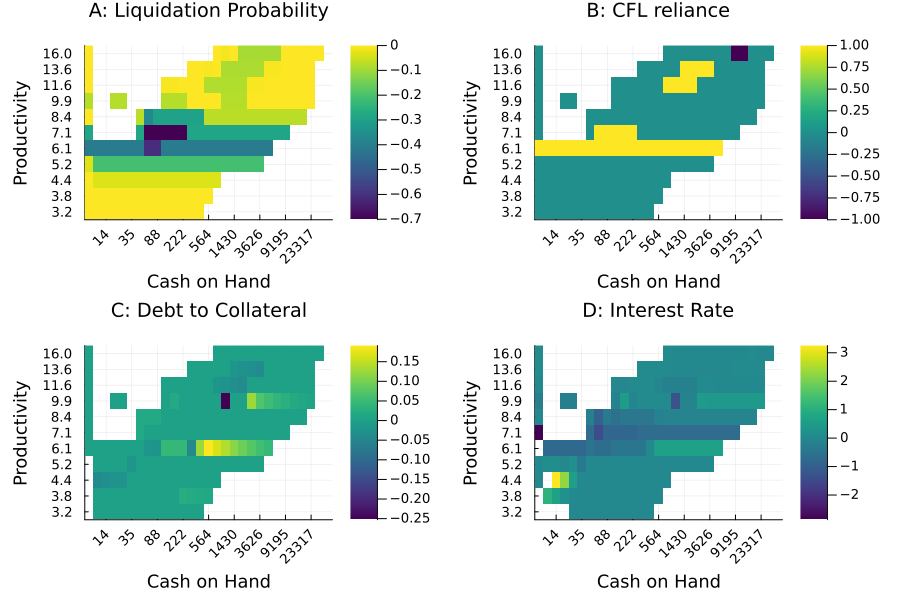
\includegraphics[width=1\textwidth]{C:/Users/szjud/OneDrive/Asztali gép/EBCs/CFL-git/reform.png}
    \caption{\small The change in equilibrium outcomes following the reform. The y-axis represents the productivity state, and the x-axis the cash on hand value. The color intensity corresponds to the magnitude of the change. The non-colored tiles correspond to states in which the mass of firms is less than 0.01\% of the total in the stationary equilibrium. Panel A shows the change in liquidation probability, Panel B shows the change in reliance on CF-based debt, Panel C shows the change in debt-to-collateral ratio and Panel D shows the change in interest rates. }
    \label{chart:poleffects}
\end{figure}

\noindent Figure \ref{chart:poleffects} illustrates the impact of the smaller reform across different productivity states and cash-on-hand values - and figure \ref{chart:extpoleffects} in the appendix presents the effects of the 'extreme reform'. Non-colored tiles correspond to states in which the mass of firms is less than 0.01\% of the total in the stationary equilibrium. Panel A shows the change in liquidation probability following the reform. The most and least productive firms are largely unaffected by the reform. This pattern arises because former are unlikely to liquidate even before the implementation of the reform, whereas the latter are unlikely to reorganize even after the reduction of fixed costs. Hence the reform has the greatest impact on firms with relatively high productivity, though not at the very top of the distribution (the lowest 11 productivity states are omitted from Figure \ref{chart:poleffects}). For these firms, however, liquidation probability drops substantially, by 30 to 70 percentage points.   \vspace{3mm} \\
The rest of the equilibrium outcomes reflect the changes in ex-ante liquidation probability. Panel B shows the change in reliance on CF-based debt. Although the model can, in principle, accommodate any CF-reliance between zero and one, under the current model assumptions firms always choose a corner solution. Hence, CF-reliance is either zero or one in the model and the bright yellow tiles correspond to firms that switch from asset-based borrowing to CF-based borrowing as a result of the reform. Panels C and D show changes in the debt-to-collateral ratio and interest rates, respectively. The firms most affected by the reform either borrow at a lower interest rate or realize higher debt-to-collateral ratios.  \vspace{3mm} \\
Table \ref{tab:percentage_changes} summarizes the effects of the reform in alternative model specifications, in which firms can access only asset-based debt (AB-only) or only CF-based debt (CF-only). For reference, I also report the effects in the baseline model. The `AB-only' case is implemented by setting lenders' payoffs in reorganization to zero, while the `CF-only' case is implemented by setting lenders' payoffs after liquidation to zero. In both cases, the model is recalibrated to match the targeted moments of average liquidation probability, debt-to-collateral ratio and interest rate. 

\begin{table}[H]
    \centering
    \begin{tabular}{lccc}
    & \textbf{AB only} & \textbf{Baseline Model} & \textbf{CF only} \\    
    \toprule
    Total firm mass & 0\% & 4.2\%  & 20.91\%  \\  
    Mean employees & 0\% & -4.04\%  & -17.29\%   \\  
    Productivity (Y/L) & 0\% & 1.34\%  & 2.40\%  \\  
    Capital Int. (K/L) & 0\% & 0.26\%  & 0.68\%  \\  
    Wage & 0\% & 1.34\%  & 2.40\%  \vspace{2mm}  \\  
    Pr. Liquidation & -18.06 pp & -18.43 pp  & -21.69 pp \\  
    Debt/Collateral & 0 pp & 3.07 pp  & 5.82 pp  \\  
    Interest rate & 0 pp & -0.45 pp  & 0.71 pp  \\  
    CF reliance & 0 pp & 21.2 pp  & 0 pp  \\    
    CF share & 0 pp & 6.83 pp  & 0 pp  \\  
    \bottomrule
    \end{tabular}
    \caption{Reform effects in recalibrated model versions where only asset-based debt is available (AB only), and only CF-based debt is available (CF only). The baseline model is also reported as reference.}
    \label{tab:percentage_changes}
\end{table}

\noindent When only asset-based debt is available, the change in liquidation probability does not influence other equilibrium outcomes.\footnote{The reform’s effects are considered solely through credit frictions. Facilitating reorganizations may have broader implications beyond credit markets, which are not considered here.} Since most macro-finance models do not account for CF-based debt financing, this case illustrates the effects of the reform in `standard' models of credit frictions. This result may explain why ex-ante liquidation probability have received scant attention in prior research. In contrast, when only CF-based debt is available, the model overestimates the impact of the reform. In the baseline case, firms that are expected to liquidate under financial distress can fall back to asset-based borrowing, since this loan-type is not exposed to liquidation risk. In the absence of this backstop on the cost of external finance, the model over-emphasizes the effects of liquidation probability on equilibrium outcomes. For further discussion on how liquidation probability affects interest rates and debt financing strategies, see section \ref{sec:appliqrisk} in the appendix. 

\section{The Small Business Reorganization Act}
In February 2020, the Small Business Reorganization Act (SBRA) introduced Subchapter V to Chapter 11 of the U.S. Bankruptcy Code. This reform was based on the recognition that traditional Chapter 11 bankruptcy is often prohibitively costly and time-consuming for small firms. The SBRA includes several provisions aimed at making the reorganization process more accessible for small businesses.
\begin{enumerate}
    \item \textit{Elimination of Creditor Committees}. No automatic requirement for a creditors' committee, reducing administrative costs and simplifying the bankruptcy process.   
    \item \textit{Simplified Creditor Cramdown}. A reorganization plan can be confirmed without unanimous creditor approval (provided the Bankruptcy Court deems it fair and equitable), reducing delays and legal costs.
    \item \textit{Elimination of the Absolute Priority Rule}. Firm owners can retain equity without fully repaying unsecured creditors, making restructuring more feasible.
    \item \textit{Reduced Reporting and Disclosure Requirements}. Fewer financial disclosure obligations, lowering compliance costs.
    \item \textit{Streamlined Reorganization Process}. Deadlines for filing and confirming a plan are shortened, reducing the time and expense of reorganization.
    \item \textit{Appointment of a Subchapter V Trustee}. A trustee is assigned to assist the development of a consensual reorganization plan, without assuming control of the business.
\end{enumerate}

\noindent Evaluating the effects of these provisions is beyond the scope of this paper. However, the structural model offers valuable predictions about certain aspects of this reform. In particular, I assess SBRA's focus on small firms relative to a universal policy and the reduction of creditor control over the reorganization process.  \vspace{3mm} \\
\textit{Eligibility is limited to small firms}. \\ 
The reduced reporting requirements, streamlined reorganization process, and appointment of a Subchapter V trustee (provisions 4 to 6) lower the administrative and time costs of reorganization. These provisions are closely aligned with baseline reform discussed in section \ref{sec:results}. However, the debt limit for SBRA eligibility has never exceeded $\$7.5$ million, effectively excluding large firms from this type of bankruptcy.\footnote{At its introduction, Subchapter V eligibility was limited to businesses with no more than approximately $\$2.75$ million in debt. Shortly after, this debt limit was temporarily increased to $\$7.5$ million in response to the COVID-19 pandemic, and was later reduced to an original (inflation-adjusted) threshold of around $\$3$ million in June 2024.} I model this aspect of the SBRA as a targeted reduction in the fixed costs of reorganization. The second column of table \ref{tab:percentage_changes2} show the equilibrium effects of a targeted policy that reduces fixed reorganization costs by half for small firms only. \vspace{3mm} \\
Compared to the universal reform, the equilibrium effects of the targeted policy are somewhat smaller but not significantly so. As discussed in the section \ref{sec:model}, fixed reorganization costs disproportionately burden small firms meaning that the reduction of these costs also chiefly benefits these firms. Hence, the results in table \ref{tab:percentage_changes2} confirm that exluding large firms from the SBRA has limited effects on the effectiveness of the reform. It is not likely that these reforms only affects the fixed costs of reorganization. Therefore in table ... in the appendix, I also consider a targeted reduction in variable costs. Since fixed costs are the primary barrier to reorganization for small firms, this change has negligible effects on equilibrium outcomes.  \vspace{3mm} \\
\textit{Reducing creditor control over the reorganization process} \\
The SBRA enhances debtor rights by limiting creditor control over the reorganization process. The elimination of creditor committees, allowing deveiations from absolute priority rule and the simplified creditor cramdown (provisions 1 to 3) all point to this direction. Since these measures reduce lenders' bargaining power, I represent these in the model as a reduction of lenders' ability to seize future cash flow through the debt-renegotiation process (reduction in $\phi_c$). Figure ... shows the effects of a targeted and a universal reduction in creditor control. 


\begin{table}[H]
    \centering
    \begin{tabular}{lccc}
     & \textbf{Universal} & \textbf{Targeted} & \textbf{Control Reduc.} \\    
    \toprule
    Total firm mass & 4.2\%  & 2.20\% & 1.55\%  \\  
    Mean employees & -4.04\%  & -2.15\% & -1.58\%   \\  
    Productivity (Y/L) & 1.34\%  & 0.97\% & 0.25\%  \\  
    Capital Int. (K/L) & 0.26\%  & 1.25\% & 2.80\%  \\  
    Wage & 1.34\%  & 0.97\% & 0.25\%  \vspace{2mm}  \\  
    Pr. Liquidation & -18.43 pp  & -11.92 pp & -17.90 pp \\  
    Debt/Collateral & 3.07 pp  &  1.53 pp & -0.86 pp  \\  
    Interest rate & -0.45 pp  & -0.35 pp & -0.20 pp  \\  
    CF reliance & 21.2 pp  & 20.58 pp & -3.47 pp  \\    
    CF share & 6.83 pp  & 2.23 pp & -54.51 pp  \\  
    \bottomrule
    \end{tabular}
    \caption{Reform effects in recalibrated model versions. Baseline refirm: fixed costs are halved. Targeted reform: the fixed costs of reorganization are halved only for small firms. Creditor control reducing reform: the fixed costs are halved but so is creditors ability to extract future cash flows.}
    \label{tab:percentage_changes2}
\end{table}



\section{Conclusion}

This paper demonstrates that reorganization costs raise liquidation risks and limit access to cash flow-based debt for small but productive firms, which has significant consequences for broader macroeconomic outcomes. The empirical analysis establishes that ex-ante liquidation risk increases credit spreads on cash flow-based loans, limiting access to credit for firms that lack sufficient collateral. The structural model quantifies the macroeconomic implications of these credit frictions. High reorganization costs increase liquidation probability for small firms, limits their access to CF-based debt, which contributes to credit misallocation, suppresses firm entry and yield aggregate productivity losses. \vspace{3mm} \\
The model findings also shed light on the broader implications of bankruptcy policy reforms, such as the Small Business Reorganization Act (SBRA). By reducing reorganization costs, policymakers can enhance credit allocation, alleviate financing constraints and ultimately improve aggregate productivity. While targeted policies that facilitate small firm reorganization help reduce liquidation risk and expand access to CF-based debt, shifting reorganization costs to lenders may have unintended effects, leading them to limit CF-based lending preemptively. These results highlight the importance of designing bankruptcy frameworks that promote borrower flexibility without compromising creditor protection.

\newpage

\appendix
\section*{Appendix}
\section{Model Solution \label{sec: qualitative analysis}}

In the structural model discussed above, optimal firm policies and the interest rate schedule offered by the lender are jointly determined. That is, lenders adjust interest rates to firm policies, while firms choose these policies in light of the interest rate schedule offered to them. To address issue, I adopt the following solution algorithm:\footnote{This follows Corbae and D'Erasmo (2021).}
\begin{enumerate}
    \item Set $q^0 = 0$ of inverse interest rate for all firm policies and calculate the value of the firm, $V_{cont}(k,b,\varepsilon)$, the optimal firm policies $k', b', \tau'$ as well as the exit and liquidation policies. 
    \item Calculate the following: the probability of default $P_D$, the probability of liquidation in default $\gamma$, the liquidation value; $\phi_A (1-\delta) k'$ and the reorganization value; $\phi_c V (x', \varepsilon')$ given $q^0$, for each state-policy pair
    \item Update interest rate associated with the state-policy pair, taking into account the default and liquidation probability and lenders in-default payoffs. This gives $q^1$. 
    \item Repeat $1-3$ until the optimal policies and interest rates do not change in successive iterations - that is, $ (k^{i},b^{i},\chi_d^{i},q^{i}, V^{i}) = (k^{i-1},b^{i-1},\chi_d^{i-1}, q^{i-1}, V^{i-1}) $.
\end{enumerate}
This algorithm is relatively robust, but it comes at a great computational cost. It usually takes around 15 to 20 iterations to converge, which implies the same number separate solutions of firm optimization (step number 1) and updating the interests rate schedule (step number 2 and 3). 

\section{Costs of Lending against Future Cash Flows \label{sec:fixed costs}}
In section \ref{sec: The lender's problem}, I adopt a highly stylized description of fixed costs: these are imposed only on households which allows me to match the high liquidation probability associated with small corporations. In the interest of keeping the model simple, I do not impose a separate fixed costs on lenders. In practice however, the default resolution process often involves a lengthy negotiation between debtors, creditors, and courts, which imposes significant costs on every involved parties. Hence, when in-default payments are expected through reorganization, the lender must take into account the legal, personnel and time expenses of this process. \vspace{3mm} \\
However, maintaining a cash flow-based debt contract may impose significant costs on the lender even in the normal course of business. Asset-based contracts only require occasional audits of the borrower's assets. In contrast, cash flow-based contracts necessitate that the lender carries out its `due diligence' on an ongoing basis. The apparatus to maintain this monitoring activity may impose significant expenses on creditors.\footnote{This type of cost shares some similarities with the costly state verification first proposed by Towsend (1979).} More generally, such costs could be thought of as all additional expenses lenders face on a regular basis, when they deviate from standardized asset-based contracts.
\vspace{3mm} \\
In summary, evidence would also support for imposing additional fixed costs on creditors for lending against future cash flows. In fact, it would be possible to coin the central trade-off of the model in terms of these fixed cost. In this scenario, asset-based debt would provide the benefit of not having to monitor borrower performance and would offer a quick and cost-effective way of retrieve in default payments. Conversely, CF-based contracts would allow to potentially retrieve a share of the continuation value, but it would impose significant fixed costs on the lender. I do not include this mechanism in the model, as it would produce very similar results to the baseline setup. However, it is important to note that these fixed costs may influence lenders to favor one loan type over another.


\section{The Small Business Reorganization Act \label{sec:A2}}

The Small Business Reorganization Act (SBRA), effective February 19, 2020, introduced Subchapter V to Chapter 11 of the Bankruptcy Code aiming to make bankruptcy reorganizations more accessible and cost-effective for small businesses. Its' key reforms include granting debtors exclusive rights to propose reorganization plans, thereby barring creditors from submitting competing proposals. The SBRA also eliminates US Trustee fees and the formation of creditor committees, further simplifying the process. Moreover, the removal of the absolute priority rule allows small business owners to retain equity even without fully repaying unsecured creditors, provided they commit projected disposable income to debt repayment over a three-to-five-year period. \vspace{3mm} \\
However, these debtor-friendly changes often come at the expense of creditors.  Eliminating the absolute priority rule reduces the bargaining power of unsecured (CF-based) creditors, while provisions for stretched administrative payments delay their compensation. In conclusion, the SBRA represents a policy shift aimed at incentivising and facilitating small business reorganizations, albeit at the expense of creditor interests in certain cases. In the model, I summarize SBRA as an exogenous reduction in the fixed costs of reorganization and also as a reallocation of these costs to the lender. Although this summary is highly stylized, it captures the effect of policies that aim to reduce the liquidation risk of small firms. 

\section{Data appendix \label{sec:A3}}
\subsection{Compustat and Capital IQ}
Compustat is a comprehensive, financial database maintained by S\&P Global. It offers standardized firm-level information on publicly traded companies compiled from financial statements, regulatory filings and other financial reports. I use the quarterly tables in Compustat North America and drop firms that are not headquartered in the US. Moreover, I exclude financial corporations (SIC code 6000 to 6799) and utility providers (SIC code 4900-4999). \vspace{3mm} \\
S\&P Capital IQ offers an extensive array of debt-level statistics. The two datasets can be connected via the unique firm a identifier (GVKEY), moreover Capital IQ covers most of the Compustat firms and yields consistent firm-level debt data after the aggregation of debt contracts. Although Capital IQ covers most major economies, I only focus on US corporations, due to limitations introduced by Compustat. Both of these datasets are accessed through Wharton Research Data Services (WRDS). \vspace{3mm} \\
Although both datasets provide high quality reports, reporting differences necessitate some manipulation of the data. Since monetary variables are often reported in the native currency, I bring all observations to USD. Moreover, Capital IQ reports data points in different units (units, thousands or millions). To be consistent to Compustat, I bring all observations to millions of units. It must also be ensured that each observation is uniquely identified by the combination of year, quarter, and debt ID. This may be violated for various reasons, for instance, debt facilities are often reported twice (once with the total accessible debt and once with the currently outstanding amount). In these cases, I only consider the outstanding amount. Moreover, in some cases the parent firms nad the subsidiaries are both included in the data. In these cases, I only consider parents in order to maintain observations at the highest consolidation level. \vspace{3mm} \\
In some instances, debt contracts go missing only to reappear a few quarters later. If this gap between observations is no more the 4 quarters, I use linear interpolation to fill up the data. These cases are relatively rare as they only amount to approximately 7\% of the total sample. To ensure the alignment of consistent observations, I aggregate debt-level data from CapitalIQ to the firm level and cross-reference it with the debt information reported by Compustat. I drop any observations where there is a disparity of more than 20\% between the two datasets. This discards around 8\% of the original sample. Tables \ref{tab:COMPS} and \ref{tab:CAPIQ} summarize Capital IQ and Compustat variables, including their original names and definitions in these datasets. \vspace{3mm} \\
Moreover, I explore bankruptcy data drawn from the Integrated Database (IDB) maintained by the Federal Judicial Center (FJC). This is a comprehensive resource containing detailed records of federal court cases in the United States. It includes data on civil, criminal, bankruptcy, and appellate cases from the Administrative Office of the US Courts. For this analysis, only bankruptcy cases under Chapters 7 and 11 are considered, focusing on the period from 2010 to 2023, which corresponds to the period covered by the Capital IQ - Compustat dataset. 

\begin{table}[htbp]    

    \centering
    \begin{tabular}{ll}
    \toprule
    Variable & Capital IQ \\
    \midrule
    Loan value & dataitemvalue \\
    Decimal of the value & unittypeId \\
    Currency of issuance & issuedCurrencyId \vspace{3mm} \\
    \multicolumn{2}{l}{\textbf{Used for contract classification}} \\
    Description of the contract & capitalstructuredescription \\
    Type of the debt contract & capitalstructuresubtypeid \\
    Debt description in text & descriptiontext \\
    Secured dummy & securedtypeid \\
    Seniority & leveltypeid \vspace{3mm} \\
    \multicolumn{2}{l}{\textbf{Firm-level aggregated variables}} \\
    Total debt value & Sum of all contracts value \\
    AB value & Sum of all AB debt \\
    CF value & Sum of all CF debt \\
    CF-share & CF value / Total debt \\
    \bottomrule
    \end{tabular}
    \caption{\small Variables downloaded from Capital IQ and their corresponding name in WRDS.}
    \label{tab:CAPIQ}

\end{table}


\begin{table}[htbp]    
\centering
\renewcommand{\arraystretch}{1.5} % Increase the vertical spacing of rows
\resizebox{\textwidth}{!}{%
\begin{tabular}{lp{5cm}p{7cm}} 
\toprule
Variable & Compustat Definition & Description \\
\midrule
Total debt & dlcq+dlttq & Long-Term Debt + Debt in Current Liabilities \\
Leverage & (dlcq+dlttq)/atq & Total debt / Total Assets \\
Collateral & ppentq+invtq+rectq & Total Property, Plant and Equipment (net) + Receivables + Inventory \\
Pledgeability & (ppentq+invtq+rectq)/atq & Collateral / Total Assets \\
Interest coverage & oibdpq / xintq & Operating income before depreciation / Interest related expenses \\
Investment & capxq-sppeq & Capital expenditures - Sale of Property \\
Investment rate & (capxy - sppey) / l.ppegtq & Investment / Lag of Total Property, Plant and Equipment (gross) \\
Equity & atq-ltq & Total assets / Total liabilities \\
Net debt & dlcq+dltq-chq & Total debt - Cash Holdings \\
Liquidity & chq/atq & Cash Holdings / Total Assets \\
Assets & atq & Total Assets (book value) \\
Liabilities & ltq & Liabilities (book value) \\
Revenue & revtq & Total quarterly revenue \\
EBITDA & oibdpq & quarterly EBITDA measure \\
Employees & emp & Total number of employees (thousands) \\
Industry spec. & sic & SIC code \\
Credit rating & spcsrc & S\&P credit rating \\
Age & from Capital IQ & Current year - Year founded + 1 \\
\bottomrule
\end{tabular}
}
\caption{\small Variables downloaded from Compustat and their corresponding name in WRDS.}
\label{tab:COMPS}
\end{table}

\begin{table}[h!]
    \centering
    \label{tab:IDB}
    \begin{tabular}{ll}
    \toprule
    Variable & Description \\ 
    \midrule
    SNAPSHOT & Date variable \\ 
    SNAPFILE & 1 if filed in the period \\ 
    SNAPPEND & 1 if still pending in the period \\ 
    SNAPCLOS & 1 if ended in the period \\ 
    ORGFLDT & Original filing date \\ 
    CLOSEDT & Closing date \\ 
    CRNTCHP & Current bankruptcy chapter \\ 
    CLCHPT & Closing bankruptcy chapter \\ 
    EASST & Estimated total assets \\ 
    ELBLTS & Estimated total liabilities \\ 
    \bottomrule
  \end{tabular}
  \caption{\small Variables downloaded from IDB and their corresponding name in WRDS.}
\end{table}
    
\subsection{Summary Statistics \label{sec:sumstat}}

\begin{table}[H] 
    \centering
    \resizebox{0.95\textwidth}{!}{%
    \begin{tabular}{lrrrrrr}
    \multicolumn{7}{l}{\textbf{Firm-Level Summary Statistics}} \\
    \hline
        & \textbf{Mean} & \textbf{p10} & \textbf{p25} & \textbf{Median} & \textbf{p75} & \textbf{p90} \vspace{1mm} \\
    Total Assets (millions USD) & 5235.16 & 11.39 & 73.11 & 582.60 & 2696.20 & 9567.60 \\
    Qtr. Revenue (millions USD) & 1073.75 & 0.18 & 8.77 & 109.62 & 551.79 & 1891.00 \\
    Employees (thousands) & 11.93 & 0.03 & 0.15 & 1.37 & 6.91 & 22.85 \\
    Firm Age (years) & 44.61 & 9 & 16 & 30 & 59 & 109 \\
    Cash to Assets (Liquidity) & 0.17 & 0.01 & 0.03 & 0.09 & 0.21 & 0.46 \\
    Debt to Assets (Leverage) & 0.30 & 0.03 & 0.12 & 0.27 & 0.43 & 0.61 \\
    Debt to Collateral & 0.51 & 0.11 &  0.26 &  0.52 & 0.75 & 0.89 \\ 
    Asset Pledgeability (\%) & 47.21 & 9.32 & 23.48 & 46.91 & 70.53 & 85.81 \\
    Total debt (millions USD) & 1817.35 & 1.06 & 8.33 & 132.69 & 960.90 & 3562.65 \\
    CF-share & 0.45 & 0.00 & 0.00 & 0.40 & 0.92 & 1.00 \\
    Average Maturity (years) & 6.7 & 1.4 & 4.0 & 6.1 & 8.6 & 12.2 \\
    Average Interest Rate (\%) & 4.9 & 0.3 & 2.7  & 4.6 & 6.8 & 9.2 \\
    Average Spread & 2.9  & 0 & 0.6 & 2.3 & 4.4 & 6.9 \\
    \hline
    \end{tabular}%
    }
    \caption{\small Summary Statistics - non-financial corporations between 2010Q1 and 2023Q2}
    \label{tab:sumstat1}
\end{table}

\begin{table}[H]
    \centering
    \resizebox{0.95\textwidth}{!}{%
    \begin{tabular}{lrrrrrr}
    \multicolumn{7}{l}{\textbf{Debt-Level Summary Statistics}} \\
    \toprule
      	& \textbf{Mean} & \textbf{p10} & \textbf{p25} & \textbf{Median} & \textbf{p75} & \textbf{p90} \vspace{1mm}\\
    Contract Value (millions USD) & 334.53  & 0.16 & 2.24 & 48.24 & 396.00 & 859.22 \\ 
    Maturity (years) & 9.275 & 2.50 & 4.50 & 7.00 & 10.00 & 20.00 \\
    Interest Rate (\%) & 5.79 & 2.12 & 3.60 & 5.25 & 7.38 & 10.00 \\
    Credit Spread & 4.03  & 0.87 & 1.88 & 3.45 & 5.49 & 8.06  \\
	\bottomrule
    \end{tabular}%
    }
    \caption{\small Summary Statistics - debt contracts between 2010Q1 and 2023Q2}
    \label{tab:sumstat2}
\end{table}

\section{Additional Empirical Analyses}


\subsection{Classification of Debt Contracts \label{sec:classification}}
Classification into asset-based and CF-based debt is conceptually different from the notion of secured and unsecured debt.\footnote{Even though they may be strongly correlated. This leads Gonzalez and Sy (2024) to treat them as empirical equivalents. This approach is acceptable when blanket liens are rarely used  as is case for the Spanish corporate credit market.} Security establishes priority in bankruptcy, dictating who `queues first' to collect payments if the firm goes under. Conversely, the distinction between asset-based and cash flow-based debt refers to the economic determinants of lenders' in-default payoffs. When debt is backed by specific physical assets, lenders' in-default payoffs reflect the liquidation value of these items. In the case of CF-based debt, no specific physical asset serves as collateral meaning that in-default payoffs are chiefly determined by the future cash-flows of the borrower. \vspace{3mm} \\
I follow the classification strategy of Lian and Ma (2021). Debt contracts that are not explicitly secured by specific physical assets are classified as cash flow-based debt. Hence, debentures and other unsecured debt contracts are counted towards this category. Bonds and notes are also considered cash flow-based debt, as they are typically unsecured or secured against future cash flows - through liens on substantially all assets or equity. The exceptions to this are mortgage bonds, which are backed by real estate, and thus fall under the category of asset-based debt. Similarly, capitalized leases are also classified asset-based. Finally, I consider debt contracts that are categorized as `term loans', `revolving credit' or `other borrowings' by Capital IQ. Depending on the specifics of the contract, these can be asset-based and cash flow-based debt as well. To remain conservative about the share of cash flow-based debt, I classify these instruments as asset-based, unless they are unsecured. \vspace{3mm} \\ 
In line with the previous findings of Lian and Ma (2021) and Öztürk (2022), the total outstanding debt volume that can be classified as CF-based is relatively stable around 75\%. However, starting from 2019, this share drops significantly - from 79\% in 2018Q4 to 71\% 2019Q4 - and it does not fully recover until the end of the sample. It is not clear what causes this abrupt shift in aggregate CF-share. One explanation could be the Covid-induced economic crisis. However, this leaves the initial drop, which happen before the pandemic had a substantial impact on North American economies unexplained. It is not feasible to compare these results with prior studies, as none have studied this time period.

\begin{figure}[H]  % [h] indicates placing the image here
    \centering
    \textbf{\large The Share of CF-based Debt Over Time \vspace{2mm}} \\  % This acts as a title
    \label{chart:CFLshare}
    \includegraphics[width=1\textwidth]{C:/Users/szjud/OneDrive/Asztali gép/EBCs/CFL-git/Latex codes/Plots/CFshare.png} \\
     \caption{\small The share CFL debt to total debt, by volume between 2010Q1 and 2023Q3}
\end{figure}

\subsection{Determinants of Credit Spreads \label{sec:credit spreads}} 
In this section, I study the firm-level determinants of credit spreads for asset-based and cash flow-based debt contracts. The structural model proposed in this paper accounts for endogenous variation in external finance premia, meaning that the empirical results presented here can be studied against predictions of the structural model. Firms with higher EBITDA and larger total asset value benefit from lower credit spreads on both loan-types. Prior analyses that interpret credit market frictions as either asset-based or earings-based limits to borrowing. In contrast, this result suggests that size and profitability are important determinants of these frictions no matter the form of borrowing. Another important determinant of credit spreads is leverage, which has a large, positive effect on credit spreads for both loan-types. Firm age has a significant, negative effect on credit spreads, suggesting that strong creditor-debtor relationships can help reduce the cost of external finance.  \vspace{3mm} \\
The coefficient estimates for number of employees are not consistent across specifications. This variable has limited economic impact, which indicates that total assets is a sufficient measure of firms size. Consistent with the idea that lender perception plays a key role in cash flow-based borrowing, worse credit ratings significantly increase credit spreads for this type of debt. In contrast, credit spreads for asset-based debt are influenced only when credit ratings signal the state default or a high risk of it. Sector fixed effects have mostly insignificant impact on credit spreads for asset-based debt, which is partly due to accounting for pledgeability in the model. For cash flow based debt, sector differences are more significant, yet they remain relatively unimportant determinants of credit spread variations. \vspace{3mm} \\
`CF-share' measures the extent to which a firm relies on cash flow-based debt as a fraction of total debt. It is defined as 
\begin{equation*}
    \text{CF-share} = \text{CF-based Debt Value} \  / \  \text{Total Debt Value}.
\end{equation*}
CF-share is correlated negatively with spreads of cash flow-based debt and positively with spreads of asset-based debt, suggesting that firms self-select into these loan-types based on their relative costs. This underlines that debt financing is jointly determined with the credit spreads that firms eventually face. 

\subsubsection{Limiations of Empirical Analyses \label{sec:credit spreads}} 
Empirical analyses of credit spreads and firm characteristics face significant limitations. Firms adjust their debt financing strategies based on credit conditions, which are influenced by firm characteristics. In turn, this affects the external finance premia they eventually face. This feedback effect is likely to introduce endogeneity bias. Moreover, certain determinants of credit frictions are difficult to observe. In this paper, I highlight the probability of liquidation, but other factors such as assets specificity (Kermani and Ma, 2020) or the quality of accounting practices and court enforceability (Lian and Ma, 2021) are similarly hard to measure. Therefore, identification of causal relationships between firm characteristics and credit spreads is not possible without relying on natural experiments. The structural model discussed below aims to make up for these limitations. 

\begin{table}[H]
    \centering
    \caption{The Determinants of Credit Spreads}
    \label{tab:spread_table_full}
    \resizebox{\textwidth}{!}{%
    \begin{tabular}{lcccccc}
    \toprule
    & \multicolumn{2}{c}{All contracts} & \multicolumn{2}{c}{CF contracts} & \multicolumn{2}{c}{AB contracts} \\
    \cmidrule(lr){2-3} \cmidrule(lr){4-5} \cmidrule(lr){6-7}
    \textbf{LHS}: Spread & Value & SE & Value & SE & Value & SE \\
    \midrule
    Log of EBITDA & -0.163*** & (0.011) & -0.119*** & (0.012) & -0.205*** & (0.020) \\
    Log of Assets & -0.394*** & (0.049) & -0.452*** & (0.060) & -0.321*** & (0.086) \\
    Pledgeability & -0.479*** & (0.087) & -0.046 & (0.107) & -1.013*** & (0.153) \\
    Num. Contracts  & 0.003** & (0.002) & 0.012*** & (0.002) & 0.003 & (0.004) \\
    Leverage & 1.759*** & (0.105) & 2.189*** & (0.136) & 0.963*** & (0.176) \\
    Log of Age & -0.135*** & (0.026) & -0.133*** & (0.030) & -0.147*** & (0.045) \\
    Log of Employees & -0.011 & (0.020) & -0.094*** & (0.025) & 0.084*** & (0.031) \\
    CF-share & 0.446*** & (0.064) & -0.339*** & (0.112) & 0.737*** & (0.111) \vspace{3mm} \\
    \multicolumn{7}{l}{\textbf{Industries} - baseline: Agriculture and Fishing} \\
    Construction  & 0.742*** & (0.269) & 1.246*** & (0.461) & 0.271 & (0.375) \\
    Manufacturing  & 0.280 & (0.242) & 0.641 & (0.446) & 0.124 & (0.310) \\
    Mining & 0.856*** & (0.251) & 1.020** & (0.455) & 0.728** & (0.333) \\
    Retail Trade  & 0.676*** & (0.255) & 1.234*** & (0.455) & 0.057 & (0.338) \\
    Services & 0.283 & (0.247) & 0.776* & (0.448) & -0.176 & (0.321) \\
    Public Utilities & 0.586** & (0.247) & 0.878* & (0.449) & 0.290 & (0.330) \\
    Wholesale Trade & 0.672** & (0.262) & 0.757 & (0.462) & 0.565 & (0.345) \vspace{3mm} \\
    \multicolumn{7}{l}{\textbf{Credit Ratings} - baseline: Rating: A} \\
    Rating: A+ & 0.144 & (0.095) & 0.351*** & (0.087) & -0.418 & (0.570) \\
    Rating: A- &  0.169** & (0.077) & 0.185*** & (0.065) & -0.059 & (0.363) \\
    Rating: B+ & 0.715*** & (0.071) & 0.698*** & (0.065) & 0.149 & (0.326) \\
    Rating: B & 0.207*** & (0.068) & 0.107* & (0.058) & -0.044 & (0.331) \\
    Rating: B- & 0.976*** & (0.072) & 1.159*** & (0.069) & 0.195 & (0.325) \\
    Rating: C  & 1.690*** & (0.082) & 1.613*** & (0.091) & 1.090*** & (0.327) \\
    Rating: D & 2.020*** & (0.140) & 2.429*** & (0.185) & 1.072*** & (0.362) \\
    \midrule
    Firm-level controls & Yes & & Yes & & Yes & \\
    Period fixed effects & Yes & & Yes & & Yes & \\
    Observations & 17,601 & & 10,620 & & 6,981 & \\
    R-squared & 0.285 & & 0.404 & & 0.174 & \\
    \bottomrule
    \end{tabular}%
    }
    \caption{\small Determinants of credit spreads of new issuances. Robust standard errors are reported in parentheses,  *** p$<$0.01, ** p$<$0.05, * p$<$0.1.}
\end{table}





\subsection{Robustness tests \label{sec:robustness}}

In this section, I test the robustness of the empirical results in alternative model specifications. First, I keep the same specification but replace the variable of interest with the number of \textit{secured} debt contracts. Table \ref{tab:spread_table_new} summarizes these results. Ayotte and Morrison (2009) and Blazy and Choppard (2010) argue that security backed by physical assets often incentivizes creditors to obstruct the reorganization process. This suggests that the number of secured creditors should have an even greater impact on CF-based debt contracts. Consistent with this notion, I find that the effect of secured debt contracts on credit spreads four times larger for CF-based debt, compared to the baseline case. The negative coefficient on AB-debt contract spreads is somewhat puzzling, which can be attributed to lower liquidation risk. Zhong (2021) argues that a greater threat of liquidation reduces default probability, as firms are less likely to strategically demand reorganization.


\begin{table}[H]
    \centering
    \caption{The Determinants of Credit Spreads}
    \label{tab:spread_table_new}
    \resizebox{\textwidth}{!}{%
    \begin{tabular}{lcccccc}
    \toprule
    & \multicolumn{2}{c}{All contracts} & \multicolumn{2}{c}{CF contracts} & \multicolumn{2}{c}{AB contracts} \\
    \cmidrule(lr){2-3} \cmidrule(lr){4-5} \cmidrule(lr){6-7}
    \textbf{LHS}: Spread & Value & SE & Value & SE & Value & SE \\
    \midrule
    Log of EBITDA & -0.160*** & (0.0106) & -0.108*** & (0.0121) & -0.205*** & (0.0203) \\
    Log of Assets & -0.372*** & (0.0478) & -0.404*** & (0.0584) & -0.273*** & (0.0859) \\
    Leverage & 1.826*** & (0.109) & 2.179*** & (0.137) & 1.146*** & (0.181) \\
    Pledgeability & -0.427*** & (0.0904) & -0.0790 & (0.109) & -0.847*** & (0.157) \\
    Secured contracts & 0.007 & (0.006) & 0.051*** & (0.011) & -0.021** & (0.009) \\
    \midrule
    Firm-level controls & Yes & & Yes & & Yes & \\    
    Period fixed effects & Yes & & Yes & & Yes & \\
    Observations & 17,514 & & 10,640 & & 6,874 & \\
    R-squared & 0.287 & & 0.406 & & 0.174 & \\
    \bottomrule
    \end{tabular}%
    }
    \caption{\small The main determinants of credit spreads of new issuances, when the number of secured debt contracts is taken into account. Robust standard errors are reported in parentheses,  *** p$<$0.01, ** p$<$0.05, * p$<$0.1.}
\end{table}

\noindent Calculating credit spreads is subject to uncertainty, as it is not clear interest rate the lender used as a refernce. Therefore the analyses presented in table 3 are repeated with interest rate as the dependent variable. In this specification, debt contract maturity is included alongside other firm-level controls. Table \ref{tab:intrate_table_new} summarizes these results.  The central findings remain unchanged, though the effect of the number of debt contracts on CF-based debt contracts is somewhat smaller. The negative coefficients for asset-based contracts likely reflect a stronger commitment to fulfilling the debt obligations.

\begin{table}[H]
    \centering
    \caption{The Determinants of Interest Rates}
    \label{tab:intrate_table_new}
    \resizebox{\textwidth}{!}{%
    \begin{tabular}{lcccccc}
    \toprule
    & \multicolumn{2}{c}{All contracts} & \multicolumn{2}{c}{CF contracts} & \multicolumn{2}{c}{AB contracts} \\
    \cmidrule(lr){2-3} \cmidrule(lr){4-5} \cmidrule(lr){6-7}
    \textbf{LHS}: Interest Rate & Value & SE & Value & SE & Value & SE \\
    \midrule
    Log of EBITDA & -0.127*** & (0.0106) & -0.0870*** & (0.0126) & -0.178*** & (0.0186) \\
    Leverage & 1.969*** & (0.105) & 2.218*** & (0.141) & 1.545*** & (0.164) \\
    Log of Assets & -0.348*** & (0.0528) & -0.386*** & (0.0703) & -0.206** & (0.0833) \\
    Pledgeability & -0.302*** & (0.0885) & 0.00467 & (0.116) & -0.640*** & (0.141) \\
    Num. contracts & 0.001 & (0.001) & 0.009*** & (0.001) & -0.006* & (0.004) \\
    \midrule
    Firm-level controls & Yes & & Yes & & Yes & \\    
    Period fixed effects & Yes & & Yes & & Yes & \\
    Observations & 22,652 & & 12,613 & & 10,039 & \\
    R-squared & 0.235 & & 0.335 & & 0.143 & \\
    \bottomrule
    \end{tabular}%
    }
    \caption{\small Determinants of interest rates of new issuances. Robust standard errors are reported in parentheses,  *** p$<$0.01, ** p$<$0.05, * p$<$0.1.}
\end{table}

\noindent Limiting the analysis to new issuances reduces the sample size. By using a weighted average of firm-level credit spreads as the outcome variable, it is possible to explore the variables that influence external finance premia beyond the time of issuance. Here, I consider three sub-samples: firms that borrow inly against assets, only against and cash flows as well as the entire sample. Despite relying on an entirely differnt approach to the analysis of credit spreads, the main results remain largely unchanged. 

\begin{table}[H]
    \centering
    \caption{The Determinants of Credit Spreads}
    \label{tab:spread_table_new}
    \resizebox{\textwidth}{!}{%
    \begin{tabular}{lcccccc}
    \toprule
    & \multicolumn{2}{c}{All contracts} & \multicolumn{2}{c}{CF contracts} & \multicolumn{2}{c}{AB contracts} \\
    \cmidrule(lr){2-3} \cmidrule(lr){4-5} \cmidrule(lr){6-7}
    \textbf{LHS}: Spread & Value & SE & Value & SE & Value & SE \\
    \midrule
    Log of EBITDA & -0.058*** & (0.005) & -0.009 & (0.015) & -0.192*** & (0.012) \\
    Log of Assets & -0.0286 & (0.0235) & -0.490*** & (0.0793) & -0.0338 & (0.0478) \\
    Leverage & 2.049*** & (0.0484) & 1.942*** & (0.177) & 1.909*** & (0.112) \\
    Pledgeability & -0.237*** & (0.0424) & 0.758*** & (0.154) & -0.940*** & (0.0832) \\
    Num. Contracts & 0.006*** & (0.001) & 0.026*** & (0.005) & -0.038*** & (0.006) \\
    \midrule
    Firm-level controls & Yes & & Yes & & Yes & \\
    Period fixed effects & Yes & & Yes & & Yes & \\
    Observations & 78,714 & & 8,938 & & 26,604 & \\
    R-squared & 0.144 & & 0.167 & & 0.157 & \\
    \bottomrule
    \end{tabular}%
    }
    \caption{\small The main determinants of credit spreads of new issuances, considering the number of secured debt contracts. Robust standard errors are reported in parentheses, *** p$<$0.01, ** p$<$0.05, * p$<$0.1.}
\end{table}

\section{Additional Model Results \label{sec:appmodelresults}}


\begin{figure}[H]  % [h] indicates placing the image here
    \centering  
    \textbf{\large Extreme Reform Effects on Credit Conditions \vspace{3mm} \\}   % This acts as a title
    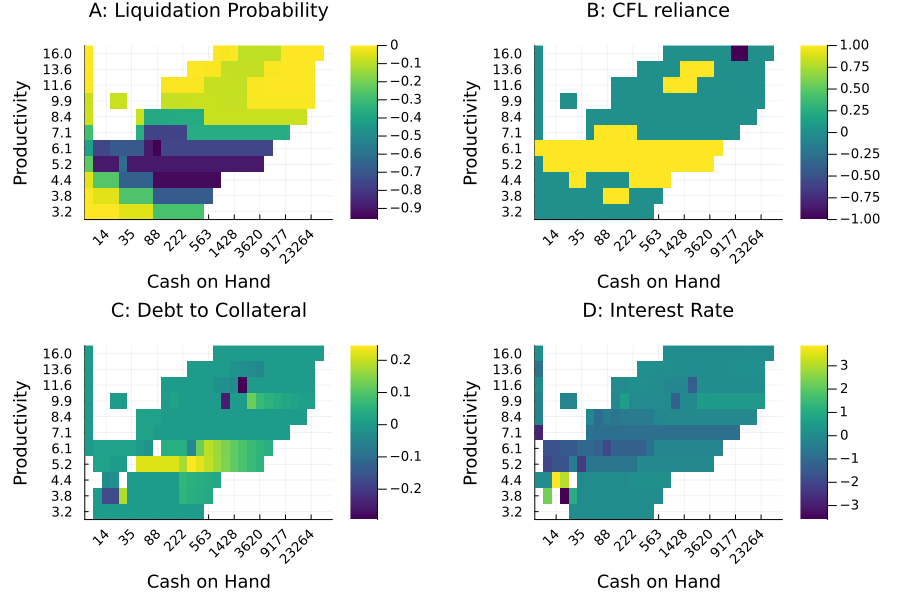
\includegraphics[width=1\textwidth]{C:/Users/szjud/OneDrive/Asztali gép/EBCs/CFL-git/large_reform.png}
    \caption{\small The change in equilibrium outcomes following the \textit{extreme} reform. The y-axis represents the productivity state, while the x-axis represents the cash on hand value, the color intensity corresponds to the magnitude of the change. The non-colored tiles correspond to states in which the mass of firms is less than 0.01\% of the total in the stationary equilibrium. Panel A shows the change in liquidation probability, Panel B shows the change in reliance on CF-based debt, Panel C shows the change in debt-to-collateral ratio and Panel D shows the change in interest rates. }
    \label{chart:extpoleffects}
\end{figure}


\subsection{Liquidation Risk and Credit Conditions \label{sec:appliqrisk}}

In this section, I present model predictions on how liquidation risks affect the cost of external finance and firms' optimal debt financing strategy. In the general equilibrium model liquidation probability does not change exogenously, therefore this exercise is based on a reduced version of the model. Based on equation \ref{eq:q}, I determine the interest rate that would support the equilibrium policies of ($k',b'$), under different liquidation probabilities. Moreover, I define the corresponding optimal reline on CF-based debt ($\tau$), based on equation \ref{eq:V_cont}. Figure \ref{chart:liqprob} presents these results for a high-productivity firm, for three different values of cash on hand. The lines are color-coded to represent the debt financing strategy of the firm, either borrowing against assets (red) or against cash flows (blue). \\

\begin{figure}[H]  % [h] indicates placing the image here
    \centering  
    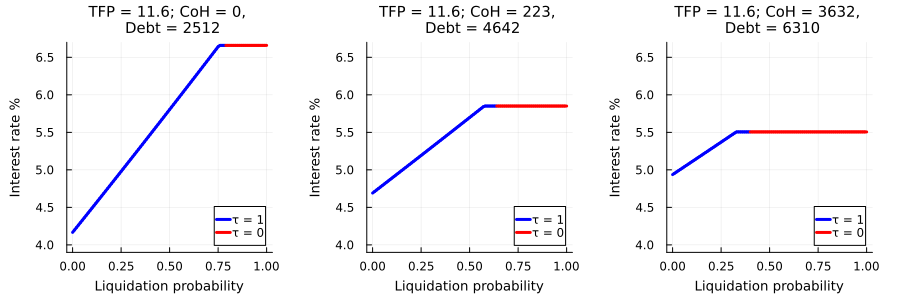
\includegraphics[width=1\textwidth]{C:/Users/szjud/OneDrive/Asztali gép/EBCs/CFL-git/GamPol.png}
    \caption{ \small External finance premium based and debt financing strategy necessary to support firms equilibrium policies. Panel A, corresponds to firms starting cash on hand, panel B. depicts expected cash on hand after one period, and panel C. is the steady-state cash on hand at the given productivity level.}
    \label{chart:liqprob}
\end{figure}

\noindent Firms enter with zero cash on hand, therefore panel A. corresponds to credit conditions upon entry. The effects of liquidation probability are largest for these firms, as they do not have private wealth to support their capital investments. Under zero liquidation probability, these firms may access CF-based financing at a 4.1\% rate. This rate increases monotonously until 75\% of liquidation probability, at which point firms transition to asset-based borrowing at a rate of 6.6\%. This represent an upper bound for interest rates, as asset-based debt contracts are not affected by liquidation probability. \vspace{3mm} \\
Panel B. corresponds to firms' expected cash on hand after one period, given optimal policy decisions. Having accumulated some wealth, these firms can access more future capital, which is associated with higher continuation value. Hence, these firms face lower interest rates across all liquidation probabilities. Hence, accumulating cash on hand limits firms' exposure to liquidation risk and higher capital stock allows these firms to fall back to asset-based debt sooner. Panel C. corresponds to the steady-state cash on hand for the given productivity. This panel shows the same decline in external finance premia across liquidation probabilities, but the overall effects are even more pronounced. \vspace{3mm} \\
Figure \ref{chart:liqprob} provides further insights into firms' debt financing frictions. First, even though age is not explicitly considered in the model, firms' lifecycle affects their credit conditions. Small but productive firms, who benefit the most from reducing liquidation risks, are almost invariably young firms, within the first three years of entry. Hence, the model predicts the reducing reorganization costs aids young firms the most. Second, although the model can accommodate any CF-reliance between zero and one, under the current assumption firms always choose a corner solution, either borrowing only against assets or entirely against cash-flows. Third, the value-maximizing debt financing strategy maximizes the inverse interest rate faced by the firm. Both of these results follow from firm value being in zero and default. 


\end{document}